\newif\ifdraft\drafttrue

\documentclass[12pt]{report}

\usepackage{palatino}
\usepackage{listings}
\usepackage{graphicx}
\usepackage{xcolor}
\usepackage{fullpage}
\usepackage{tabularx}
\usepackage{keystroke}
\usepackage{natbib}

\lstset{
  language=Python, 
  frame=lines, 
  numbers=left, 
  basicstyle=\small\ttfamily,
  aboveskip=20pt,
  belowskip=20pt
}
\lstdefinestyle{BashInputStyle}{ 
  language=bash, 
  basicstyle=\small\ttfamily,
  keywordstyle=\small\ttfamily,
  columns=fullflexible,
  keepspaces=true,
  numbers=none,
  moredelim=[l][\color{blue}]{\$},
  moredelim=[l][\color{blue}]{mininet>},
  aboveskip=20pt,
  belowskip=20pt
}
\graphicspath{ {./omnigraffle/} }

\begin{document}

\title{
\includegraphics{frenetic-logo.png}\\Programmers Guide}

\author{\Large Craig Riecke\\[3ex]
\large with \\[3ex]
%
\large Others\\[1ex]
}
\date{\LARGE \ifdraft {\bf Draft of} \fi  \today}

\maketitle

\tableofcontents{}

% !TEX root = frenetic_programmers_guide.tex

\chapter{Quick Start}

In this book, you will use Frenetic to create a full-programmable network.  For the moment, let's assume you're familiar with Software Defined Networking and the OpenFlow protocol, and just dive right in.  (If you're not, don't worry!  We'll introduce some bedrock concepts in the next chapter and explain everything that happened here.)  

\section{Installation}

There are several ways to get started with Frenetic, but the easiest is to use Frenetic VM.  Frenetic itself only runs on Linux, but the Frenetic VM will run on any host system that supports VirtualBox, including Windows, Mac OS X and practically any version of Linux itself.   Keeping Frenetic it in its own VM will keep your own system clean and neat.  Later on, if you want to install Frenetic on a bare metal Ubuntu Linux server or network device, you can use the instructions in \ref{productionalizing:install}.  

\begin{itemize}
\item Install VirtualBox from https://www.virtualbox.org/wiki/Downloads.  Use the latest version platform package appropriate for your system.  
\item Install Vagrant at http://www.vagrantup.com/downloads.  Vagrant automates the process of building VM's from scratch, and Frenetic VM uses it to build its own environment.  This is more reliable than downloading a multi-gigabyte VM file.   
\item Install Frenetic VM from https://github.com/frenetic-lang/frenetic-vm.  You can simply use the Download Zip button and unzip to an appropriate directory on your system, like frenetic-vm.  Then from a terminal or command prompt:

\begin{lstlisting}[style=BashInputStyle]
 $ cd /path/to/frenetic-vm
 $ vagrant up
 ... lots of text 
\end{lstlisting}
\end{itemize}

The build process may take 15 minutes to an hour, depending on the speed of your system and Internet connection. 

\section{What Do You Get With Frenetic VM?}

At the end of the process you will have a working copy of Frenetic with lots of useful open source infrastructure:

\begin{description}
\item[Mininet] software builds a test network inside of Linux.  
It can simulate a topology with many switches and hosts.  
Writing a network application and throwing it into production is \ldots well, pretty risky, but running it on Mininet first can be a good test for how it works beforehand.  
We'll use it throughout this book.  
\item[Wireshark] captures and analyzes network traffic.  
It's a great debugging tool, and very necessary for sifting through large amounts of data.
\item[Frenetic].  This layer provides an easy-to-use programmable layer on top of ODL.  Its main job is to shuttle OpenFlow messages between ODL and your application, and to translate the language NetKAT into OpenFlow flow tables.  We'll see the differences between the two as we go.
\end{description}

Hmmm, that's a lot of software - what do {\it you} bring to the table?  You write your network application in Python, using the Frenetic framework.  As you'll see, it's quite easy to build a network device from scratch, and easy to grow it organically to fit your requirements.  Python is fairly popular, and knowing it will give you  a head start into Frenetic programming.  But if you're a Python novice that's OK.  As long as you know one object-oriented language fairly well, you should be able to follow the concepts.  We'll introduce you to useful Python features, like list comprehensions, as we go.  

\section{An Attempt at Hello World}

So let's dive right in.  We'll set up a Mininet network with one switch and two hosts.  First you should work from the directory where you installed Frenetic VM.

\begin{lstlisting}[style=BashInputStyle]
 $ cd /path/to/frenetic-vm
\end{lstlisting}
 
Then start up the VM:

\begin{lstlisting}[style=BashInputStyle]
 $ vagrant up
 ringing machine 'default' up with 'virtualbox' provider...
==> default: Clearing any previously set forwarded ports...
==> default: Clearing any previously set network interfaces...
==> default: Preparing network interfaces based on configuration...
    default: Adapter 1: nat
==> default: Forwarding ports...
    default: 22 => 2222 (adapter 1)
==> default: Running 'pre-boot' VM customizations...
==> default: Booting VM...
==> default: Waiting for machine to boot. This may take a few minutes...
    default: SSH address: 127.0.0.1:2222
    default: SSH username: vagrant
    default: SSH auth method: private key
    default: Warning: Connection timeout. Retrying...
==> default: Machine booted and ready!
==> default: Checking for guest additions in VM...
==> default: Setting hostname...
==> default: Mounting shared folders...
    default: /vagrant => /Users/cr396/frenetic-vm
    default: /home/vagrant/src => /Users/cr396/frenetic-vm/src
==> default: Machine already provisioned. Run `vagrant provision` or...
==> default: to force provisioning. Provisioners marked to run always...
\end{lstlisting}

Then log in to the VM.  At this point your command prompt will change to {\tt vagrant@frenetic} to distinguish it
from your host machine.

\begin{lstlisting}[style=BashInputStyle]
 $ vagrant ssh
Welcome to Ubuntu 14.04.2 LTS (GNU/Linux 3.16.0-30-generic x86_64)

 * Documentation:  https://help.ubuntu.com/
Last login: Tue Oct  6 10:35:06 2015 from 10.0.2.2
vagrant@frenetic:~$ 
\end{lstlisting}

So you are now working inside an Ubuntu-based VM.  You don't really need to know Ubuntu, but just know that Mac OS and Windows commands won't necessarily work here.  

Let's start up a Mininet network with one switch and two nodes.

\begin{lstlisting}[style=BashInputStyle]
vagrant@frenetic:~$ sudo mn --topo=single,2 --controller=remote
*** Creating network
*** Adding controller
Unable to contact the remote controller at 127.0.0.1:6633
*** Adding hosts:
h1 h2
*** Adding switches:
s1
*** Adding links:
(h1, s1) (h2, s1)
*** Configuring hosts
h1 h2
*** Starting controller
c0
*** Starting 1 switches
s1 ...
*** Starting CLI:
mininet>
\end{lstlisting}

The prompt changes to {\tt mininet>} to show your working in Mininet.  
The error message {\tt Unable to contact controller at 127.0.0.1:6633} looks a little ominous, but not fatal.  

You now have an experimental network with two hosts named h1 and h2.  
To see if there's connectivity between them, use the command \lstinline{h1 ping h2} which means ``On host h1, ping the host h2.''

\begin{lstlisting}[style=BashInputStyle]
mininet> h1 ping h2
PING 10.0.0.2 (10.0.0.2) 56(84) bytes of data.
From 10.0.0.1 icmp_seq=1 Destination Host Unreachable
From 10.0.0.1 icmp_seq=2 Destination Host Unreachable
From 10.0.0.1 icmp_seq=3 Destination Host Unreachable
^C
--- 10.0.0.2 ping statistics ---
6 packets transmitted, 0 received, +3 errors, 100\% packet loss, time 5014ms
pipe 3
\end{lstlisting}

The ping gets executed over and over again, but it's clearly not working.  So we press CTRL-C to stop and 
quit out of Mininet:

\begin{lstlisting}[style=BashInputStyle]
mininet> quit
\end{lstlisting}

So by default, hosts can't talk over the network to each other.  We're going to fix that by writing a {\it network
application}.    Frenetic will act as the controller on the network, and the network application tells Frenetic how to act.

\section{A Repeater}

You write your network application in Python, using the Frenetic framework.  Mininet is currently running in our VM under its own terminal window, and we can leave it like that.   
We'll do our programming in another window, so start up another one and log into our VM:

\begin{lstlisting}[style=BashInputStyle]
 $ cd /path/to/frenetic-vm
 $ vagrant ssh
Welcome to Ubuntu 14.04.2 LTS (GNU/Linux 3.16.0-30-generic x86_64)

 * Documentation:  https://help.ubuntu.com/
Last login: Tue Oct  6 10:35:06 2015 from 10.0.2.2
vagrant@frenetic:~$ 
\end{lstlisting}

Create a tutorial directory for your use:

\begin{lstlisting}[style=BashInputStyle]
vagrant@frenetic:~$ mkdir tutorial
vagrant@frenetic:~$ cd tutorial
\end{lstlisting}

Now we'll write our first network application.
You can use your favorite Unix text editor - vim and nano are already installed, or you can install your own favorite
one with Ubuntu's {\it apt-get} commands. 
Nano is a nice editor if your feeling indecisive:

\begin{lstlisting}[style=BashInputStyle]
vagrant@frenetic:~/tutorial$ nano repeater.py
\end{lstlisting}

Now type in the following network application:

\begin{lstlisting}
import sys
sys.path.append('../src/frenetic/lang/python')
import frenetic
from frenetic.syntax import *

class RepeaterApp(frenetic.App):

    def connected(self):
        self.update( id >> SendToController("repeater_app") )

    def packet_in(self, dpid, port_id, payload):
        out_port = 2 if port_id = 1 else 1
        self.pkt_out(dpid, payload, [ Output(Physical(out_port_id)) ] )

app = RepeaterApp()
app.start_event_loop()
\end{lstlisting}

Lines 1-4 are pretty much the same in every Frenetic network application.
Similarly, lines 15-16 are similar in most cases. 
 The meat of the application is an object class named RepeaterApp, whose base class is \lstinline{frenetic.App}.
A frenetic application can hook code into different points of the network event cycle.
In our Repeater network app, the only two events we're interested in here are
\lstinline{connected}, which is fired when a switch connects for the first time to Frenetic, and 
 \lstinline{packet_in}, which is fired every time a packet
bound for a controller arrives.

The code in \lstinline{connected} merely directs the switch to send all packets to our application.
The interesting code is in \lstinline{packet_in} and implements a {\it repeater}.
A repeater is the oldest type of network device, and is sometimes called a {\it hub}. 
In a repeater, if a packet enters on port 1, it should get copied out to port 2.  
Conversely, if a packet enters on port 2, it should get copied out to port 1.
If there were more ports in our switch, we'd write a more sophisticated repeater -- one that
outputs the packet to all ports except the one on which it arrived (called the {\it ingress port}).  

\lstinline{pkt_out} is a method provided by Frenetic to actually send the packet out the switch.  It takes three 
parameters: a switch, a packet, and a policy.  
Here the policy sends the packet out to port \lstinline{out_port_id}.   

\section{Running The Repeater Application}

So let's get this running in a lab setup.  
Three programs need to be running:  Mininet, Frenetic, and our new Repeater application.  
For now, we'll run them in three separate command lines, having typed \lstinline{vagrant ssh} in each
to login to the VM.

In the first terminal window, we'll start up Frenetic:

\begin{lstlisting}[style=BashInputStyle]
vagrant@frenetic:~$ cd src/frenetic
vagrant@frenetic:~src/frenetic$ ./frenetic.native http-controller \
  > --verbosity debug
 [INFO] Calling create!
 [INFO] Current uid: 1000
 [INFO] Successfully launched OpenFlow controller with pid 3062
 [INFO] Connecting to first OpenFlow server socket
 [INFO] Failed to open socket to OpenFlow server: (Unix.Unix_error...
 [INFO] Retrying in 1 second
 [INFO] Successfully connected to first OpenFlow server socket
 [INFO] Connecting to second OpenFlow server socket
 [INFO] Successfully connected to second OpenFlow server socket 
\end{lstlisting}

In the second, we'll start up Mininet with the same configuration as before:

\begin{lstlisting}[style=BashInputStyle]
vagrant@frenetic:~$ sudo mn --topo=single,2 --controller=remote
*** Creating network
*** Adding controller
\end{lstlisting}

The following will appear in your Frenetic window to show a connection has been made:

\begin{lstlisting}[style=BashInputStyle]
 [INFO] switch 1 connected
[DEBUG] Setting up flow table
+----------------------+
| 1 | Pattern | Action |
|----------------------|
|             |        |
+----------------------+
\end{lstlisting}

And in the third, we'll start our repeater application:

\begin{lstlisting}[style=BashInputStyle]vagrant@frenetic:~$ cd tutorial
vagrant@frenetic:~/tutorial$ python repeater.py
No client_id specified. Using d7650d3aebfc4bd9a708eef1382041ba
Starting the tornado event loop (does not return).
\end{lstlisting}

The following will appear in the Frenetic window.  

\begin{lstlisting}[style=BashInputStyle]vagrant@frenetic:~$ cd tutorial
 [INFO] GET /version
 [INFO] POST /d7650d3aebfc4bd9a708eef1382041ba/update_json
 [INFO] GET /d7650d3aebfc4bd9a708eef1382041ba/event
 [INFO] New client d7650d3aebfc4bd9a708eef1382041ba
[DEBUG] Installing policy
drop | port := pipe(repeater_app) | port := pipe(repeater_app)
[DEBUG] Setting up flow table
+---------------------------------------+
| 1 | Pattern | Action                  |
|---------------------------------------|
|             | Output(Controller(128)) |
+---------------------------------------+
\end{lstlisting}

And finally, we'll pop over to the Mininet window and try our connection test once more:

\begin{lstlisting}[style=BashInputStyle]
mininet> h1 ping h2
PING 10.0.0.2 (10.0.0.2) 56(84) bytes of data.
64 bytes from 10.0.0.2: icmp_seq=1 ttl=64 time=149 ms
64 bytes from 10.0.0.2: icmp_seq=2 ttl=64 time=97.2 ms
64 bytes from 10.0.0.2: icmp_seq=3 ttl=64 time=88.7 ms
\end{lstlisting}

Ah, much better! 
Our pings are getting through.  
You can see evidence of this in the Frenetic window:

\begin{lstlisting}[style=BashInputStyle]
 [INFO] GET /d7650d3aebfc4bd9a708eef1382041ba/event
 [INFO] POST /pkt_out
[DEBUG] SENDING PKT_OUT
 [INFO] GET /d7650d3aebfc4bd9a708eef1382041ba/event
 [INFO] POST /pkt_out
[DEBUG] SENDING PKT_OUT
 [INFO] GET /d7650d3aebfc4bd9a708eef1382041ba/event
 [INFO] POST /pkt_out
[DEBUG] SENDING PKT_OUT
\end{lstlisting}

\section{Summary}

You now have a working SDN, or Software Defined Network!   Like much software, it works in layers:

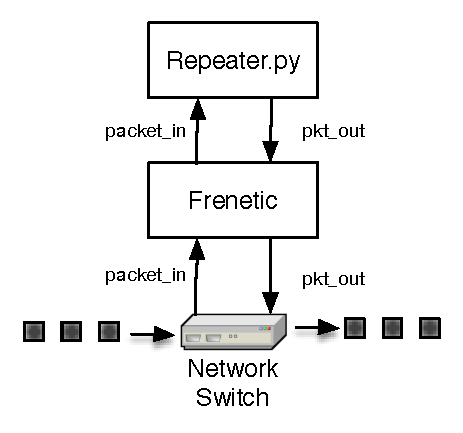
\includegraphics{frenetic_architecture}

\begin{enumerate}
\item At the bottom is your switches and wires.  In our lab setup, Mininet and OpenVSwitch is a substitute for this layer.
\item In the middle is Frenetic.  It talks the OpenFlow protocol to the switches (or to Mininet) -- this is called the Southbound interface.  It also accepts its own language called NetKAT from network applications -- this is called the Northbound interface.
\item At the very top is your network application, which you write in Python.  It defines how packets are dealt with.
\end{enumerate}

We wrote a very simple network application that emulates a network repeater.   
It responds to the \lstinline{packet_in} event coming from the switches through Frenetic when a packet 
arrives at the switch.  
And it sends the \lstinline{pkt_out} message to send the packet back out through Frenetic to the switch.  
Frenetic-vm makes installing and testing all the pieces straightforward. 
When you're done, your network application can be deployed to a real production network.

Obviously you can do much more than just simple repeating with SDN!  
We'll cover that next with some background on OpenFlow and NetKAT, the underlying language of Frenetic. 
% !TEX root = frenetic_programmers_guide.tex

\chapter{NetKAT}

Software Defined Networking, or SDN, is a huge paradigm shift in the computing world.  
Traditional networking involves 
expensive, proprietary "boxes" from major vendors, plugging them in, configuring them, and hoping they 
meet your needs.  
But traditional networking suffers from these maladies:

\begin{itemize}
\item The devices are flexible only within narrow configuration parameters. 
Special requirements, like preventing certain kinds of devices from mobility, or configuring 
the spanning tree to prefer certain paths, are either impossible or expensive.
\item While the devices are powered by software, there's no workable way to examine the underlying code or prove it's correct.  
\item Upgrades tend to be the forklift-variety, since mixing and matching old and new hardware is a dicey proposition
\ldots not to mention mixing hardware from different vendors.
\item Configuration is not easily automated. 
Solutions are often proprietary, require special programming languages, and are not interchangeable.
Because of this, modern data center virtualization is more difficult.
\item Adding support for new protocols is slow and expensive.
\end{itemize}

With SDN, data centers can step off the proprietary network treadmill.  
Its a shift similar to the personal computer revolution of the 1980's.
Before that, IBM and similar mainframes controlled the computer space, and required the same kinds of 
forklift upgrades networks do.
The IBM Personal Computer opened up the architecture to competitors, who could then design and 
build extensions
that made it more useful.
This created a snowball effect, with hardware extensions like the mouse and Ethernet cards opening the way 
for new software like Microsoft Windows and the Netscape browser.

SDN opens network devices in a similar manner, allowing them to be extended and manipulated in interesting,
user-defined ways.
Although the term SDN has been hijacked to mean many things, it most often refers to OpenFlow-enabled 
network software and devices.
OpenFlow is an open protocol defined by the Open Network Foundation that manipulates the control 
plane of a network intermediary.  

Frenetic is an OpenFlow controller, meaning it talks the OpenFlow protocol to network intermediaries.  
In turn, it exposes an API that can be used to write network programs easily.
It works with any network intermediary that understands the OpenFlow 1.0 protocol -- 
both hardware devices like the HP 2920 and software ``devices'' like Open vSwitch.  
So let's take a brief look at OpenFlow itself.

\section{Introduction to OpenFlow}

Every network device -- from the lowliest repeater, to firewalls and load balancers, all the way up to the most complex router -- has two conceptual layers:

\begin{description}
\item[The data plane] performs actions on packets.   
It manipulates headers, copies packets to outgoing (or egress) ports, or drops packets.
It consults control tables - MAC address tables, ARP caches, OSPF tables, etc. - to guide it.  
\item[The control plane] manipulates the control tables themselves.
People, in turn, may manipulate the control plane through configuration software.
Or packets may do it: specialized ones like OSPF neighbor exchange, ARP requests, or just examining plain ol'
packets themselves.
But they never actually touch the packets.
\end{description}

This separation is only conceptual.
You'd be hard pressed to open a network device, point to a chip and say, "That's the data plane."
It helps in understanding a device, though, because they have different goals:

\begin{description}
\item[The data plane]'s job is to move data as quickly as possible.
It relies more on fast table lookups than complex algorithms.
\item[The control plane] works more flexibly, yet conservatively.
Control tables should not change often, and when they do, appropriate checks and balances should be applied to
ensure the data plane keeps working.  
For example, the Spanning Tree Protocol (or STP) ensures packets are routed along the shortest path with no
loops.  
Calculating the spanning tree is the control plane's job, as its complex. 
But once that's calculated, the data plane can use it to forward packets quickly.
\end{description}

A traditional network device looks like this. 
The control plane is closed and contained fully within the box.

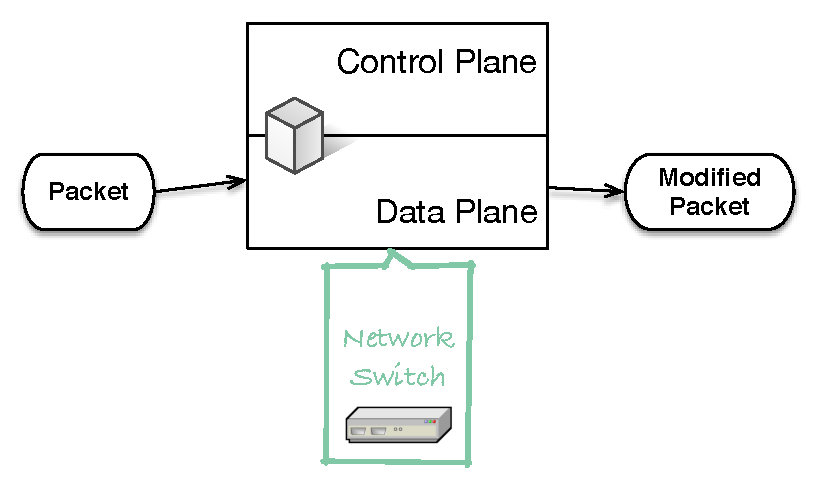
\includegraphics{traditional_device_planes}

The OpenFlow protocol makes the control plane \textit{programmable}.
Rather than relying on the entire program being inside the box, you write a program that advises the control plane
and runs outside the box.
It's like an advisor that makes aribtrarily complex control table manipulations.  
The programmable piece runs on any standard computer, and is collectively called the \textit{controller}.  

The controller can be written in any language and run on any computer \ldots the only requirement is it must speak the
OpenFlow protocol to the device.  
You can think of these two pieces working in a tandem through an OpenFlow conversation:

\begin{description}
\item[Device:] I just got a packet, but I don't know what to do with it.
It came in port 3 from Ethernet mac address 10:23:10:59:12:fb and it's going to mac address 5c:fb:12:59:10:23.
\item[Controller:] OK.    
I'll memorize that the 10:23:10:59:12:fb address is on port 3.
But I don't know which port has a device with address 5c:fb:12:59:10:23.
So just send it out all ports on the switch except port 3.  
\item[Device:] OK. \ldots Ooops, here's another packet I don't know what to do with.  
It came in port 5 from Ethernet mac address 5c:fb:12:59:10:23 and it's going to mac address 10:23:10:59:12:fb.
\item[Controller:]  Oh yeah.  
That looks like a reply.  
I'll memorize that the 5c:fb:12:59:10:23 address is on port 5.
Meanwhile, I know the destination is on port 3.  
Install a rule so all packets going to that mac address go out port 3, then forward this packet out port 3 as well.  
\item[Device:] OK!
\item[Controller:] How many packets have went out port 3, by the way?
\item[Device:] 82,120.
\item[Device:] (To itself) I just saw a packet destined for Ethernet mac address 10:23:10:59:12:fb:5c, but I have a rule for dealing with it.  I'm gonna send it out port 3.  
\end{description}

OpenFlow boils down control plane functionality to a common core set of actions.
A list of rules and actions that can be handled in the device itself are kept in a \textit{flow table}.
Any complex decisions that can't be handled independently by the control plane may be offloaded to the controller.  
In a well-designed Software Defined Network, the controller gets involved only when necessary.
After all, the conversation between the device and the controller takes time, and anything that can 
eliminate this conversation makes the packets go faster.
So in the example above, a rule for any packets going to 10:23:10:59:12:fb:5c to be output on port 5 keeps all the processing on the switch, and out of the controller.  
That makes it really fast.  

So, central to the OpenFlow model is the \textit{flow table}.  
Flow tables have \textit{entries}, sometimes called \textit{flow rules}, that are consulted for making decisions.
A sample flow table might look like this:

\bigskip
\begin{tabularx}{6in}{|l|l|c|}
\hline\hline
Match & Actions & Priority
\\ \hline
dl\_src = 10:23:10:59:12:fb:5c, & OFPAT\_OUTPUT(9) & 100
\\
dl\_type = 0x806 & &  
\\ \hline
nw\_src = 128.56.0.0/16, & OFPAT\_SET\_DL\_DST(5c:fb:12:59:10:23), & 90 
\\
dl\_type = 0x800 & OFPAT\_OUTPUT(1) &
\\ \hline
Wildcard & OFPAT\_OUTPUT(Controller) & 1
\\ \hline\hline
\end{tabularx}

\bigskip

The main components of a flow entry are:

\begin{description}
\item[A match] specifies patterns of packet header and metadata values.
OpenFlow 1.3 defines 40 different fields to match: some popular ones are the Input Port, 
the Ethernet Destination mac address, and the TCP destination port.
The match values can either be exact (like 10:23:10:59:12:fb:5c above) or wild carded (like 128.56.0.0/16 for a
particular Ip subnet).
\item[Actions] tell what to do if the match occurs.  
Instructions can apply actions (send a packet out a port, or write some header information, 
or send a packet to the controller), 
invoke groups (like a function call in a programming language), or set variables.
\item[A priority] defines the order that matches are consulted.  
When more than one entry matches a particular packet, the entry with the highest priority wins.
\end{description}

In our example above, the controller installed a flow entry matching Ethernet Destination 10:23:10:59:12:fb:5c, 
and an instruction applying the action "Output it through Port 3".

OpenFlow's flow table model is \textit{abstract}.
An OpenFlow device is not necessarily going to find a RAM chip with the matches, 
instructions and priorities \ldots although a pure software switch like Open vSwitch might mirror it quite closely.
Instead, the controller asks the device to install entries, and the device accommodates it by placing entries in its
own tables.
For example, a real network device might have an L3 table that matches subnets with the various ports that have
IP gateways.
A programmer, knowing this table exists, can write instructions that match on those ports, and place it directly in the
table accordingly.

Suppose you wanted to write your own controller from scratch.  
You could do that just by talking the OpenFlow protocol.
Let's say you wrote this program in Node.js and placed it on the server "controller.example.com", 
listening on TCP port 6653.
Then you'd just point your OpenFlow network device at controller.example.com:6653.
Then your program could install flow table entries into the network device over the OpenFlow protocol.

Hmmm.
Sounds pretty easy, but \ldots

\section{OpenFlow is Difficult}

From a programmer's perspective, a table looks awfully primitive.  
``That's not code, that's data,'' you might say.
But a table is very easy for switch hardware to interpret, and the faster they can interpret and carry 
out rules, the faster the packets travel.  
It's like machine language, where the CPU interprets simple instructions very quickly, and even in parallel.

You don't program in machine language most of the time, though, and you shouldn't have to program directly in
OpenFlow tables.
Why not?  

\begin{itemize}
\item The set of matches and actions is very limited
\item They are difficult to modularize and compose
\item They are difficult to prove correct.  
\end{itemize}

Programming OpenFlow tables directly, you begin to find out the subtle missing details:

\begin{itemize}
\item You can only match packets with $=$.   There's no $\neq$.
\item There is an implicit And in all match rows and an implicit Or between all rules, but you can't be 
more flexible than that.    
\item Matching against a set of values requires you to write one rule per value.  
\end{itemize}

Because tables often have thousands of rules, they are difficult to construct and debug.  
In the programming world, \emph{modularization} aids both of these problems since smaller units of code
are easier to understand.  

OpenFlow tables have no inherent grouping mechanism, but we could simply modularize them by 
constructing small tables that do target packet processing.  Smoosh them together
into one big OpenFlow table when we're done, right?  

But as the paper \citet{frenetic} points out in section IIA, even simple modules can be difficult
to \emph{compose}.   Suppose your SDN switch needed to do two things: repeat all traffic, but drop all
HTTP packets coming from port 2 (a makeshift firewall).  The repeater table might look something like this:

\bigskip
\begin{tabularx}{4in}{|l|l|c|}
\hline\hline
Match & Actions & Priority
\\ \hline
in\_port=1 & OFPAT\_OUTPUT(2) & 200
\\ \hline
in\_port=2 & OFPAT\_OUTPUT(1) & 100
\\ \hline\hline
\end{tabularx}

\bigskip

And the firewall table might look like this:

\bigskip
\begin{tabularx}{4in}{|l|l|c|}
\hline\hline
Match & Actions & Priority
\\ \hline
in\_port = 2, & None & 100
\\
tp\_src\_port = 80, &  & 
\\
dl\_type = 0x800, & &
\\
nw\_proto = 0x1 & &
\\ \hline\hline
\end{tabularx}

\bigskip

If we simply smooshed the two tables together, the firewall rule would never fire because the first rule in 
the repeater table overshadows it.  In this case, reordering the priorities might work, but it's impossible to 
do this correctly without a spec to guide it.  

Finally, it's difficult to reason about OpenFlow tables.
While it's true that the set of possible packets is a finite set, it's still a large set.  One could loop
over all header values (200 bits worth in an OpenFlow 1.0 structured packet) 
and give the corresponding actions.  But it's tough to actually enumerate all these cases.

Frenetic obeys mathematically-defined rules about packets, and its algorithms are provably correct, which 
you can see in the paper \citet{DBLP:journals/corr/SmolkaEFG15} 
And as outlined in \citet{Foster:2015:CDP:2775051.2677011}, you can prove properties like loop-freeness and
connectivity about NetKAT programs.  

\section{Predicates}

No matter what controller you use, underneath it all, you still have OpenFlow tables.
How does the Frenetic controller improve things? 

Other SDN controllers like OpenDaylight, RYU, and Beacon force you to manipulate 
OpenFlow tables directly.  
Frenetic works at a higher abstraction level.  
Here, instead of writing programs that directly call OpenFlow primitives, you write programs in 
the NetKAT language.
These programs are called \emph{network applications} or more succinctly \emph{net apps}.

Frenetic's main job is to compile NetKAT predicates and policies into OpenFlow flow tables.  
It directly communicates with the switch hardware (southbound) and to your net apps (northbound).
Net apps talk to Frenetic with good ol' fashioned HTTP, REST, and JSON.
The JSON-based NetKAT dialect is available to anyone, and any programming language that can talk HTTP and 
JSON can talk to Frenetic.
In this manual, we use the Python bindings for NetKAT because they're easy to use and extend, and they
come bundled with Frenetic.  
This saves you from dealing with the esoterica of HTTP communication and JSON formatting.  

So let's look at NetKAT predicates first.  
A \textit{predicate} is a clause used to match packets.
The base language is pretty straightforward:

\bigskip
\begin{tabularx}{6in}{|c|X|}
\hline\hline
\texttt{SwitchEq($n$)} & Matches packets that arrive on switch $n$, where $n$ is the Datapath ID of the switch.  
\\ \hline
\texttt{PortEq($n$)} & Matches packets that arrive on port $n$.  Generally ports are numbered 1-$m$, where $m$ is the
number of interfaces, but they don't need to be consecutive.  
\\ \hline
\texttt{EthSrcEq($mac$)} & Matches packets whose Ethernet Mac source address is $mac$, which is a string in the standard form $nn:nn:nn:nn:nn:nn$ where the $n$'s are lowercase hexadecimal digits.
\\ \hline
\texttt{EthDstEq($mac$)} & Matches packets whose Ethernet Mac destination address is $mac$.
\\ \hline
\texttt{VlanEq($vlan$)} & Matches packets whose VLAN is $vlan$, and integer from 1-4096.  Packets without a VLAN are never matched by this predicate.
\\ \hline
\texttt{VlanPcpEq($p$)} & Matches packets whose VLAN Priority Code Point is $p$.  Packets without a VLAN are never matched by this predicate.
\\ \hline
\texttt{EthTypeEq($t$)} & Matches packets whose Ethernet Type is $t$, where t is a 32 bit integer.  Popular values of $t$ are 0x800 for IP and 0x806 for ARP.  
\\ \hline
\texttt{IPProtoEq($p$)} & Matches packets whose IP Protocol is $p$, a number from 0-255.  
Popular values are 1 for ICMP, 6 for TCP and 17 for UDP.  
This match only makes sense when EthTypeEq(0x800, 0x806) (IP or ARP). 
\\ \hline
\texttt{IPSrcEq($addr$, $mask$)} & Matches packets whose IP source address is $addr$.  
If $mask$ is provided, a number from 1-32, this matches all hosts on a network whose first $mask$ bits match the host.
If it's omitted, the entire address is matched -- i.e. only one IP host.  
This match only makes sense when EthTypeEq(0x800, 0x806) (IP or ARP). 
\\ \hline
\texttt{IPDstEq($addr$, $mask$)} & Matches packets whose IP destination address is $addr$.  
Follows same rules as IpSrcEq.
\\ \hline
\texttt{TCPSrcPortEq($p$)} & Matches packets whose TCP source port is $p$, an integer from 0-65535.
\\ \hline
\texttt{TCPDstPortEq($p$)} & Matches packets whose TCP destination port is $p$, an integer from 0-65535.
Popular values are 80 for HTTP, 22 for SSH, and 443 for SSL.  
\\ \hline\hline
\end{tabularx}

\bigskip
If you're familiar with OpenFlow, this list should look familiar to you -- it's the same list of fields you can 
use in an OpenFlow flow table.
One special case is SwitchEq, matching a switch id, which we'll talk about in a second.  

For each rule, OpenFlow allows only one kind of boolean operator: AND.  
If the OpenFlow rule specifies match criteria $p1$, $p2$, \ldots, $pn$, the packet must match $p1$ AND $p2$
AND \ldots AND $pn$.  
NetKAT is much more expressive, allowing the following boolean operators between predicates:

\bigskip
\begin{tabularx}{6in}{|c|X|}
\hline\hline
\texttt{$p1$ \& $p2$} & Matches packets that satisfy $p1$ AND $p2$
\\ \hline  
\texttt{And([$p1$, $p2$, \ldots, $pn$])} & 
Matches packets that satisfy all the predicates: $p1$ AND $p2$ AND \ldots AND $pn$
\\ \hline  
\texttt{$p1$ $\vert$ $p2$} & Matches packets that satisfy $p1$ OR $p2$
\\ \hline  
\texttt{Or([$p1$, $p2$, \ldots, $pn$])} & 
Matches packets that satisfy one of the predicates: $p1$ OR $p2$ OR \ldots OR $pn$
\\ \hline  
\texttt{\textasciitilde $p1$} & Matches packets that DO NOT satisfy $p1$
\\ \hline  
\texttt{Not($p1$)} & Synonym for \texttt{\textasciitilde $p1$}
\\ \hline\hline
\end{tabularx}

\bigskip

The precedence is the same as for most Boolean operators in normal programming languages: 
\lstinline{Not}, then \lstinline{And}, then \lstinline{Or}.  

A bunch of predicates, stitched together with Boolean operators, can be used wherever a simple predicate is used.
Furthermore, predicates can be assigned to Python variables.
So here are some examples in Python code:

\begin{lstlisting}
import sys
sys.path.append('../src/frenetic/lang/python')
import frenetic
from frenetic.syntax import *

# Note this program doesn't actually do anything

# Match packets from a particular mac address
src_match = EthSrc("10:23:10:59:12:fb:5c")

# Match packets from a particular port that are either IP or ARP packets
port_ip_arp_match = PortEq(9) & EthType(0x800, 0x806)

# Matches packets from a particular port on switches 2 or 3 only
port_switch_match = PortEq(8) & SwitchEq(2, 3)

# Matches broadcast packets or packets from a particular port 
# or packets with a particular Vlan
all_criteria = [ EthSrc("ff:ff:ff:ff:ff:ff"), PortEq(1), VlanEq(2345) ] 
brd_or_port_match = Or( all_criteria ) 

\end{lstlisting}

One predicate requires some explanation: \lstinline{SwitchEq}.  
An OpenFlow flow table belongs to one and only one switch, but a NetKAT program belongs to every
switch connected to that controller.  
So a predicate tagged with \lstinline{SwitchEq} will limit a particular match to a particular switch.
Any predicates that don't have a \lstinline{SwitchEq} predicate will apply to \textit{all} switches in the network.

Finally, there are a few special predicates:

\bigskip
\begin{tabularx}{6in}{|c|X|}
\hline\hline
\texttt{id} & Matches all packets
\\ \hline  
\texttt{drop} & Match no packets
\\ \hline\hline
\end{tabularx}
\bigskip

Why would you need these?  
They're useful for "catch all" rules that appear last in a list.
A good example is our repeater, where we had an id rule that matched all packets and
forwarded them to the controller.

\section{Policies}

NetKAT predicates are useless by themselves.  
To make them work, you need to form them into NetKAT \textit{policies}.
A policy is like a command.  
Often they are compiled down to OpenFlow actions, and in fact there's a lot of overlap between the two
concepts.
But just as NetKAT predicates are more powerful than OpenFlow matches, NetKAT policies are more
powerful than OpenFlow action lists.

\bigskip
\begin{tabularx}{6in}{|c|X|}
\hline\hline
\texttt{Filter($p$)} & Select packets that match NetKAT predicate p, and quietly forget the rest  
\\ \hline
\texttt{SetPort($n$)} & Set the output port for the packet to port $n$.    
\\ \hline
\texttt{SendToController($tag$)} & After all actions have been performed, send packet to controller with tag $tag$    
\\ \hline
\texttt{SetEthSrc($mac$)} & Set Ethernet Mac source address to $mac$
\\ \hline
\texttt{SetEthDst($mac$)} & Set Ethernet Mac destination address to $mac$.
\\ \hline
\texttt{SetVlan($vlan$)} & Set packet VLAN to $vlan$.  Note this is not a Vlan push - it overwrites whatever 
Vlan is in the packet (if there is one).  
\\ \hline
\texttt{SetVlanPcp($p$)} & Set VLAN Priority Code Point to $p$.
\\ \hline
\texttt{SetEthType($t$)} & Set Ethernet Type to $t$, where t is a 32 bit integer.
\\ \hline
\texttt{SetIPProto($p$)} & Set IP Protocol to $p$.    
This action is only done when EthTypeEq([0x800, 0x806]) (IP or ARP). 
\\ \hline
\texttt{SetIPSrc($addr$)} & Set IP source address to $addr$.  Note there is no mask here, as in the equivalent predicate.  
This action is only done when EthTypeEq([0x800, 0x806]) (IP or ARP). 
\\ \hline
\texttt{SetIPDst($addr$)} & Set IP destination address to $addr$.  
Follows same rules as SetIpSrc.
\\ \hline
\texttt{SetTCPSrcPort($p$)} & Sets TCP source port to $p$.
\\ \hline
\texttt{SetTCPDstPort($p$)} & Sets TCP destination port to $p$.  
\\ \hline\hline
\end{tabularx}
\bigskip

Note that \texttt{Set} policies mirror each Eq predicate, so for example the predicate \texttt{VlanEq($vlan$)} has a matching
\texttt{SetVlan($vlan$)}.
The exception is \texttt{Switch}.  
This fields is not physical fields in a packet header - rather, it is metadata that OpenFlow fills in ``invisibly''
in a packet.
So you can't set it to a particular value, like you can other header fields.
To send a packet to a different switch, you also use \texttt{Send}, but you are restricted to switches that are directly
connected to the current switch, and you must know out which port to send it (e.g. you must know the topology).
We'll cover strategies for dealing with this in \ref{spanning_tree}.
 
And just as you can combine predicates with Boolean operators, you can combine policies with NetKAT 
policy operators:

\bigskip
\begin{tabularx}{6in}{|c|X|}
\hline\hline
\texttt{$pol1$ $\vert$ $pol2$} & Copy the packet and apply both $pol1$ and $pol2$ to it.   
Also known as \textit{parallel composition}.
\\ \hline  
\texttt{Union([$pol1$, $pol2$, \ldots, $poln$])} & 
Copy the packet $n$ times and apply policy $pol[i]$ to copy $i$
\\ \hline  
\texttt{$pol1$ >> $pol2$} & Apply the policy $pol1$ to the packet, then apply $pol2$ to it
Also known as \textit{sequential composition}.
\\ \hline  
\texttt{Seq([$pol1$, $pol2$, \ldots, $poln$])} & 
Apply each of the policies $pol1$, $pol2$, \ldots, $poln$ to the packet, in order 
\\ \hline  
\texttt{IfThenElse($p$, $pol1$, $pol2$)} & If packet matches predicate $p$, then apply policy $pol1$, or else
apply $pol2$.  
Either $pol1$ or $pol2$ is applied, but never both.
Equivalent to \texttt{Filter($p$) >> $pol1$ $\vert$ Filter(\textasciitilde$p$) >> $pol2$}
\\ \hline\hline
\end{tabularx}

\bigskip

The \texttt{>>} should look familiar to C++ programmers. 
Like in C++, the \texttt{>>} operator changes a piece of data, then forwards it to the next step in the chain, one
after the other.
It's especially helpful in I/O, where you build a string from pieces, then send it to the output device (file or screen) as the
last step.
The $\vert$ symbol is somewhat like the equivalent in UNIX shell programming: the components actually run in parallel.
However, unlike $\vert$, in NetKAT you are actually running separate copies of each policy without any connections
between them.
In other words, you don't send packets from the output of one into the input of another.

Some examples will clarify.

\section{Commands and Hooks}

The truth is, just like NetKAT predicates, NetKAT policies don't do anything by themselves.
And so we come to the last level of a net app: commands and hooks.
Commands are instructions from the net app to the switches (via Frenetic).  
OpenFlow calls these \emph{controller-to-switch messages}.  
Hooks are instructions from the switches to the net app (again, via Frenetic), and OpenFlow
calls these \emph{switch-to-controller messages.}

The commands are:

\bigskip
\begin{tabularx}{6in}{|c|X|}
\hline\hline
\texttt{pkt\_out($sw$, $payload$,} & Send a packet out switch with DPID $sw$.  
\\
\texttt{$plist$, $inport$)} & We'll describe this in detail below.
\\ \hline  
\texttt{update($policy$)} & 
Update all switches with the given NetKAT policy.
This is the equivalent of setting the OpenFlow flow tables all in one shot.  
\\ \hline  
\texttt{port\_stats($sw$, $port$)} & Get statistics for a particular switch and port. 
\\ \hline  
\texttt{query($label$)} & Get user-defined statistics associated with a particular label. 
We'll cover this in \ref{chapter:statistics}.
\\ \hline  
\texttt{current\_switches()} & Gets a list of DPID's of all current, operating switches, and the operating
ports for each.  
This is most useful in the \texttt{connected()} hook.  
\\ \hline  
\texttt{config($compiler\_options$)} & Set Frenetic compiler options.  
This is an instruction to Frenetic, not the switch. 
\\ \hline\hline
\end{tabularx}

\bigskip
You call commands in your net app through plain ol' Python method calls, e.g. \texttt{self.update($policy$)}.  

The hooks are:

\bigskip
\begin{tabularx}{6in}{|c|X|}
\hline\hline
\texttt{connected()} & Called when Frenetic has finished startup and some (perhaps not all) 
switches have connected to it. 
\\ \hline
\texttt{packet\_in($sw$, $port$, $payload$)} & 
 A packet has arrived on DPID $sw$, port $port$ and either the matching Policy had a SendToController policy, or
 the packet matched no rules and the TableMiss rule forwards TableMiss packets to the controller.
 This is described in detail below.
\\ \hline  
\texttt{switch\_up($sw$)} & Called when a switch has been initialized and is ready for commands.  
Some switches send this message once every 5 minutes or some user-defined interval, and it doesn't necessarily
mean it was down before this.
\\ \hline  
\texttt{switch\_down($sw$)} & Called when a switch has been powered-down gracefully.
\\ \hline  
\texttt{port\_up($sw$, $port$)} & Called when a port has been activated.
\\ \hline  
\texttt{port\_down($sw$, $port$)} & Called when a port has been de-activated - most of the time, that means the link
status is down, the network cord has been unplugged, or the host connected to that port has been powered-off.
\\ \hline\hline
\end{tabularx}

\bigskip
Your net app may be interested in one or more of these hooks.
To add code to it, you write a \emph{handler} which implements the hook's signature.
Following Python conventions, it must be named exactly the same as the hook.
However, you don't need to provide handlers for every hook.
If you don't provide one, Frenetic uses its own default handler -- in the case of \texttt{connected()}, for example, it
merely logs a message to the console.  

We'll see most of these commands and hooks used in the next few chapters.  
But since \texttt{pkt\_out()} and \texttt{packet\_in()} are crucial to net apps, we'll describe them first here.

\subsection{The packet\_in Hook}

\texttt{packet\_in()} is used to inspect network packets.  
Note that \emph{not all packets} coming in through all switches 
arrive here -- indeed, if they did, your controller would be
horribly slow (as our Repeater example is, but we'll see how to improve it in a bit.)
Packets arrive here in one of two ways:

\begin{itemize}
\item It may match an OpenFlow rule with the action \texttt{OFPAT\_OUTPUT(OFPP\_CONTROLLER)}
also known in NetKAT as \texttt{SendToController}.
\item It may not match any OpenFlow rule.  
In OpenFlow 1.0, the default action is to send the packet to the controller.
In OpenFlow 1.3, the default action is to drop the packet, but it can be configured to send it to the controller 
instead.  
\end{itemize}

Once at the controller, Frenetic will deliver the packet to \texttt{packet\_in()}. 
The default handler will simply log a message and drop the packet, but of course that's not very interesting.

The handler is called with three parameters:

\bigskip
\begin{tabularx}{6in}{|c|X|}
\hline\hline
\texttt{sw} & The DPID of the switch where the packet arrived.
\\ \hline
\texttt{port} & The port number of the port where the packet arrived.
\\ \hline
\texttt{payload} & The raw packet data.
\\ \hline\hline
\end{tabularx}

\bigskip
There are two formats for the packet data: \emph{buffered} or \emph{unbuffered}.
Most switches will only send unbuffered data, meaning the entire network packet - header and data - will be 
transferred to the controller.
Unbuffered data can be held at the controller, changed and resent, dropped, multiplied into many different packets, or 
any arbitrary action without penalty.  

Buffered data, on the other hand, exchanges flexibility for some efficiency.
Only a subset of buffered packet data is sent to the controller - the amount is configurable, but defaults to 128 bytes which is usually enough for the Ethernet and IP headers.  
If packets are large, or the channel between the switch and controller is slow, this can save much precious time.
The buffered packet will wait at the switch until it either gets changed and sent (through \texttt{pkt\_out} in 
the case of Frenetic), or explicitly dropped, or dropped due to timeout.  

Although buffering data sounds like a good idea, it requires greater care on the net apps part to prevent
duplicate packets, race conditions, and so on.
It's also possible that truncated packets become unparseable - for example, if they get cut off in the middle of
the IP header.
Because of this, very few OpenFlow switches support buffering at all.  
If capacity is an issue, it's better to send as few packets to the controller as possible.
A judicious use of NetKAT policies in the flow table will ensure this.  

If you don't need to examine any packet data, you can simply drop $packet$, or pass it directly to \texttt{pkt\_out},
as we did in our Repeater app:

\begin{lstlisting}
...
class RepeaterApp(frenetic.App):

...
    def packet_in(self, dpid, port_id, payload):
        out_port = 2 if port_id = 1 else 1
        self.pkt_out(dpid, payload, [ Output(Physical(out_port_id)) ] )

...
\end{lstlisting}

Here, we merely send the payload out unchanged.  
If it came in as buffered data, it will be sent out as buffered data.
If it came in unbuffered, it will be sent out unbuffered.  
Pretty simple.
And in the cases where all you want to decide in the controller which ports to send out a packet, this
is all the infrastructure you need.

If you need to examine the payload, you'll need some assistance.
The payload is the raw network packet data, not parsed or translated at all.
So for the Ethernet Source address, for example, you'd need to examine bytes 14 through 19 
(byte ordering starts at 0).  
Working at this low-level is exceedingly error prone.

So Frenetic leverages the RYU Packet library.
RYU is an open source project spearheaded by NTT (Nippon Telephone and Telegraph) and its Python packet
parsing library is very solid and complete.

Frenetic provides a simple API on top of RYU Packet.

\begin{lstlisting}
# You must import the proper protocol from the RYU packet library to use it
from ryu.lib.packet import ethernet, arp
...
    def packet_in(self, dpid, port_id, payload):
        ethernet_packet = self.packet(payload, 'ethernet')
        src_mac = ethernet_packet.src
        if ethernet_packet.ethertype = 0x806:
          arp_packet = self.packet(payload, 'arp')
          src_ip = arp_packet.src_ip

...
\end{lstlisting}

\texttt{p = packet($payload$, $protocol$)} turns the raw $payload$ into a parsed packet of type $protocol$.  
From there, the fields of $p$ are the parsed values of that protocol.  
You can think of $p$ as a view into $payload$ with the $protocol$ lens attached.  
In the example above, for example, $payload$ is both an Ethernet packet and an ARP packet, and the 
variables $ethernet\_packet$ and $arp\_packet$ provide respective views into it.   
If $payload$ is not parseable into that protocol, \texttt{None} is returned.  

A complete reference for RYU packets is available at 
http://ryu-zhdoc.readthedocs.org/en/latest/library\_packet\_ref.html, 
The following is a list of the most popular protocols and fields:

\subsubsection{ethernet}

\bigskip
\begin{tabularx}{6in}{|c|X|}
\hline\hline
\texttt{dst} & Destination mac address string, formatted as "08:60:6e:7f:74:e7" 
\\ \hline
\texttt{src} & Source mac address string 
\\ \hline
\texttt{ethertype} & Ethernet frame type.  
Popular values are 0x800 for IP version 4, or 0x806 for ARP.  
\\ \hline\hline
\end{tabularx}

\bigskip
Constructor: \texttt{ethernet.ethernet(dst, src, ethertype)}

\subsubsection{vlan}

\bigskip
\begin{tabularx}{6in}{|c|X|}
\hline\hline
\texttt{vid} & VLAN id 
\\ \hline
\texttt{pcp} & Priority Code Point 
\\ \hline
\texttt{ethertype} & Ethernet frame type.  
The outer Ethernet packet has ethertype 0x8100, so this is the ethertype of the packet's data.
\\ \hline\hline
\end{tabularx}

\bigskip
Constructor: \texttt{ethernet.vlan(pcp, vid, ethertype)}

\subsubsection{ipv4}

\bigskip
\begin{tabularx}{6in}{|c|X|}
\hline\hline
\texttt{proto} & The IP version 4 protocol.  
Popular values are  6 for TCP and 17 for UDP.
\\ \hline
\texttt{src} & Source address, a 32 bit integer 
\\ \hline
\texttt{dst} & Destination address, a 32 bit integer
\\ \hline\hline
\end{tabularx}

\bigskip
Constructor: \texttt{ipv4.ipv4(proto, src, dst)}

\subsubsection{arp}

\bigskip
\begin{tabularx}{6in}{|c|X|}
\hline\hline
\texttt{opcode} & Popular values are \texttt{arp.ARP\_REQUEST} and \texttt{arp.ARP\_REPLY}.  
\\ \hline
\texttt{src\_mac} & Source mac address string, formatted as "08:60:6e:7f:74:e7"  
\\ \hline
\texttt{src\_ip} & Source IP address, a 32 bit integer  
\\ \hline
\texttt{dst\_mac} & Destination mac address string  
\\ \hline
\texttt{dst\_ip} & Destination IP address  
\\ \hline\hline
\end{tabularx}

\bigskip
Constructor: \texttt{arp.arp\_ip(opcode, src\_mac, src\_ip, dst\_mac, dst\_ip)}

\subsection{The pkt\_out Command}

\texttt{pkt\_out} is used to send out packets from the switch.  
Most of the time, the packets you send are packets you received through \texttt{packet\_in}.
But there's nothing stopping from you sending arbitrarily-constructed packets from here as well.  

The command takes the following parameters:

\bigskip
\begin{tabularx}{6in}{|c|X|}
\hline\hline
\texttt{sw} & The DPID of the switch from where the packet should be sent.
\\ \hline
\texttt{payload} & The raw packet data, wrapped in a 
Buffered or Unbuffered object type.
\\ \hline
\texttt{policy\_list} & Python list of NetKAT policies to apply to the packet data.
\\ \hline
\texttt{in\_port} & Port ID from which to send it.
This parameter is optional, and only applies to buffered packets presumably sitting at a particular port on
the switch waiting to be released.
\\ \hline\hline
\end{tabularx}

\bigskip

The $policy\_list$ effectively tells the switch how to act on the packet.  
Most NetKAT policies are usable here including \texttt{SetIPSrc} and \texttt{SendToController}.  The
exceptions are:

\begin{itemize}
  \item \texttt{Filter} is not usable.  To optionally send or not send packets, use the packet library
  from RYU to make decisions.  
  \item \texttt{SetPort} is not available, but \texttt{Output(Physical($p$))} can be substituted.  The 
  difference is subtle.  \texttt{SetPort} can be used anywhere in a policy sequence, and can be followed
  by more packet modifications.  \texttt{Output} sends the packet out immediately, and according to OpenFlow
  it is always the last action executed if present.   
  \item Only simple policies are doable, so you can't use policy operators like \texttt{Union}, \texttt{Seq} 
  and \texttt{IfThenElse}.  Instead, you can send multiple policies in a list, where there's an implied \texttt{Seq} 
  operator between them.
\end{itemize}

What if you want to modify a packet before sending it out?  
There are actually two ways to do it, each appropriate for a particular use case:

\begin{description}
  \item[Direct Modification] where you set particular data in the packet itself, reserialize it through RYU's packet
  library API, and send it in $payload$.  
  This is the only way to modify data that's not accessible to a NetKAT policy - e.g. the IPv4 source address is
  settable by NetKAT policy \texttt{SetIPv4}, but there's no equivalent policy for the ARP opcode.  
  Direct modification is only available for unbuffered packets.
  \item[Policy Modification] is achieved through the Policy list, and is limited to modification through NetKAT
  policies.
  It can be done on buffered or unbuffered packets.
\end{description}

In general, Policy Modification is preferable since it works on all packets, and saves you the costly step of parsing and 
reserializing the packet in the controller.
For example, a common routing function is to change the destination MAC address for a next hop router.
Here's an example of doing this with Policy Modification:

\begin{lstlisting}
...
    def packet_in(self, dpid, port_id, payload):
        (next_hop_mac, next_port) = calculate_next_hop(payload)
        self.pkt_out(dpid, new_payload, 
          [ SetEthDst(next_hop_mac), Output(Physical(next_port)) ]
        )	
...
\end{lstlisting}

For those times when you need Direct Modification, here's an example of how to do it:

\begin{lstlisting}
from ryu.lib.packet import ethernet, arp
...
    def packet_in(self, dpid, port_id, payload):
        (ethernet_packet, arp_packet) = 
        	self.packet(payload, ['ethernet', 'arp'])
        # Flip a request into a reply and vice versa
        arp_packet.opcode =  \ 
          arp.ARP_REPLY if arp_packet.opcode == arp.ARP_REQUEST \
          else arp.ARP_REPLY
	# Reserialize it back into a raw packet
        new_payload = self.payload(ethernet_packet, arp_packet)
        self.pkt_out(dpid, new_payload, [ Output(Physical(1)) ])	
...
\end{lstlisting}

You can also create packets from scratch with a variation of Direct Modification.  
First create the packet views with standard RYU Packet library constructors.
Then just call \texttt{self.payload()} on them to create the raw packet and send it.  

\begin{lstlisting}
from ryu.lib.packet import ethernet, arp
...
    def send_arp_reply(port, src_mac, dst_mac, src_ip, dst_ip):
        # Immediately send an ARP reply when a port comes up.
        e = ethernet.ethernet(dst=dst_mac, src=src_mac, ethertype=0x806)
        a = arp.arp_ip(arp.ARP_REPLY, src_mac, src_ip, dst_mac, dst_ip)
	# Serialize it into a raw packet
        new_payload = self.payload(ethernet_packet, arp_packet)
        self.pkt_out(dpid, new_payload, [ Output(Physical(port)) ])	
...
\end{lstlisting}

\subsection{Buffering}

Packet buffering is often a settable option in a switch's OpenFlow configuration.  It's 
especially useful when packets are large, as in Jumbo Frames.  Most switching decisions made in 
the controller look only at the packet headers, not the data, so why should you have to send it?  By buffering the
entire packet, the switch only sends the headers to the controller.  The controller only does Policy Modifications
to the buffered packet, saving the trouble of sending all of it back.  

A buffered Packet Out \emph{must always} be preceded by a buffered Packet In.  That's because you need 
to send back two things:
the incoming port id, and the buffer id.  The switch actually has separate buffer list for every port on the switch, and 
sending it back with the proper port helps it match it to the correct buffer.   
This sequence diagram shows how it commonly works:

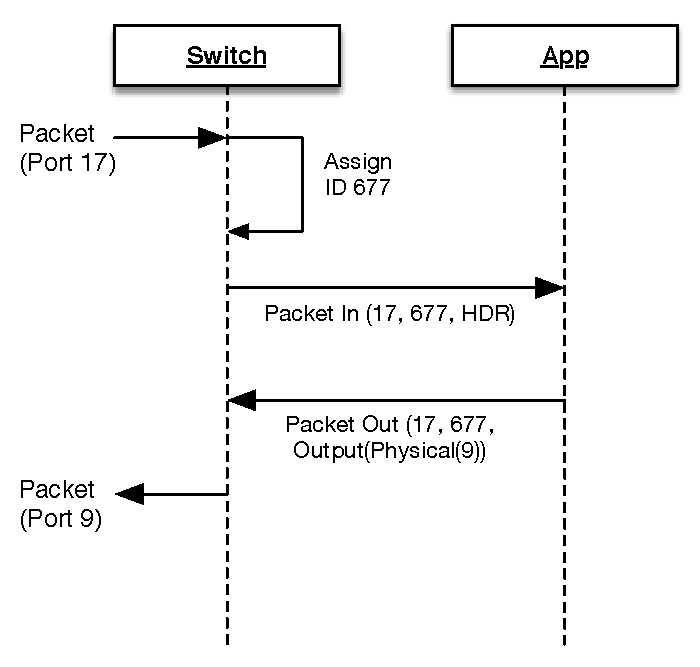
\includegraphics{buffered_pkt_happy_path}

Here, the HDR is the first 128 bytes of the packet, enough to hold the Ethernet and IP header information,
typically.  The app doesn't send any of this header information back to the switch - just the instruction
\texttt{Output(Physical(9))} to direct the switch's data plane.

What if we \emph{never} send back the Packet Out?  Buffer contents are not held indefinitely -- they timeout after a 
certain period.  At that point, the buffered packet will drop out.
If we send a Packet Out for that buffer after the timeout period, the Packet Out will generate an error (which
Frenetic ignores).    A similar fate awaits Packet Outs that fabricate a random buffer id, or send it to the
wrong port.  

So where is the buffer id in the \texttt{PacketOut} call?  It's embedded in the \texttt{payload} object.
When a \texttt{PacketIn} delivers a buffered payload, you can simply it send it back out the \texttt{PacketOut}
call, which sends the buffer id along with it.  

\section{OpenFlow Constructs Not Supported by NetKAT}

NetKAT supports the most popular features of OpenFlow 1.0.  But there a few things it can't do:

\begin{itemize}
\item It can't output to special pseudo-ports NORMAL, FLOOD, etc.  The semantics of sending to these ports
depends on the spanning tree, VLAN's, and other settings that NetKAT is not aware of, so it cannot reason
about them. 
\item It can't set the size for buffered packet data in \texttt{SendToController}.  All buffered packets
get sent with the default 128 bytes, usually enough to encapsulate the header information.
\item It can't retrieve flow table counters.  Since one NetKAT policy may expand to many OpenFlow rules, or even 
be optimized to OpenFlow Rules, there is no good way to map and retrieve this data.
\item Frenetic must talk to switches through an unsecured channel.  TLS is not supported.
\item Most controller-to-switch messages like Features, Configuration or Barrier are not supported.
\item Some switch-to-controller messages like Error, Flow Removed and Vendor are ignored by Frenetic. 
\item Some OpenFlow actions are not supported, like Enqueue.   
\end{itemize}

We haven't discussed some implemented features like Statistics yet, but those will be described in chapter \ref{chapter:statistics}.
% !TEX root = frenetic_programmers_guide.tex

\chapter{NetKAT Principles}

As we learned in the last chapter, NetKAT is a high-level Domain Specific Language for building SDN network apps.
But just as you can with any programming language, you can write incorrect, inefficient, and difficult-to-understand
NetKAT programs.
To avoid that and save you the pain of trial-and-error, this chapter presents some guiding principles for writing
your NetKAT programs.  

\newtheorem{principle}{Principle}

\section{Efficient SDN}
\label{netkat_principles:efficient_sdn}

In a nutshell, the \texttt{packet\_in()} hook receives network packets and the \texttt{pkt\_out()} command sends
network packets.  
In theory, you could use these two to implement arbitrarily-complex network clients and servers.  
You could build switches and routers, but also HTTP servers, Email servers, Database servers, or any other 
network server.  

That said, you probably wouldn't want to.
OpenFlow and Frenetic are optimized for small, very selective packet inspections and creations.  
The more packets you inspect through \texttt{packet\_in()}, the slower your controller will be, and
the more likely that packets will be dropped or sent out of sequence.  

\begin{principle}
\label{principle:controller}
Keep as much traffic out of the controller as possible.
Instead, program NetKAT policies to make most of the decisions inside the switch.  
\end{principle}

So let's go back to our Repeater application:

\inputminted{python}{code/quick_start/repeater.py}

Here, \emph{every single packet} goes from the switch to Frenetic to the net app and back out. 
That's horribly inefficient, and unnecessarily so since all the decisions can be made inside the switch.
So let's write a more efficient one.

The following code is in \codefilename{netkat_principles/repeater2.py}:

\inputminted{python}{code/netkat_principles/repeater2.py}

This program takes principle \ref{principle:controller} very seriously, to the point where \emph{no} packets 
arrive at the controller.
All of the configuration of the switch is done up front.

The \texttt{Filter(PortEq(1)) >> SetPort(2)} policy is a pretty common pattern in NetKAT.
You first whittle down the incoming flood of packets to a certain subset with \texttt{Filter}.
Then you apply a policy or series of policies, \texttt{SetPort} being the most popular.
We'll look at combining policies in section~\ref{section:combining}.

If you've worked with OpenFlow, you might wonder how the NetKAT rules get translated to OpenFlow rules.
In this example, it's fairly straightforward.
You get two OpenFlow rules in the rule table, which you can see in the Frenetic debug window:

\begin{minted}{console}
 [INFO] POST /repeater/update_json
 [INFO] GET /repeater/event
 [INFO] New client repeater
[DEBUG] Installing policy
drop | (filter port = 1; port := 2 | filter port = 2; port := 1)
[DEBUG] Setting up flow table
+-------------------------+
| 1 | Pattern | Action    |
|-------------------------|
| InPort = 1  | Output(2) |
|-------------------------|
| InPort = 2  | Output(1) |
|-------------------------|
|             |           |
+-------------------------+
\end{minted}

But this is not true in general.  
One NetKAT rule may expand into many, many OpenFlow rules.
And it may go the opposite direction to: where different NetKAT rules are combined to create one OpenFlow rule.
It's the same thing that happens with most compiled languages -- the rules that govern the compiled code
are non-trivial. 
If they were easy, you wouldn't need a compiler to do it!

There are two problems with \python{RepeaterApp2}:

\begin{itemize}
  \item It works on a two port switch, but not anything bigger.  
  And the ports absolutely have
  to be numbered 1 and 2 \ldots otherwise, the whole program doesn't work.
  \item More subtly, this program can drop packets.  
  There is a short lag between when the switches come up and the \texttt{self.update()} installs
  the policies. 
  During this lag, packets will arrive at the controller and get dropped by the 
  default \texttt{packet\_in} handler in Frenetic.   
\end{itemize}

We will correct both of these problems in section~\ref{section:stateless}.  
But first let's look at the subleties of \netkat{Union} and \netkat{Seq}.

\section{Combining NetKAT Policies}
\label{section:combining}

In our Repeater2 network app, the two rules have the \texttt{Seq} operator \texttt{>>} in them, then the two rules 
are joined together with \texttt{Union} or \texttt{|}.  
But what is the difference between the two?
When do you use one or the other?

To illustrate this, let's go back to NetKAT basics.  At the lowest level there are two types
of building blocks: filters and modifications.  

A filter takes as input a stream of packets.  Packets that match its criteria are
sent to the next policy, packets that don't match are dropped.  Two special policies, 
\texttt{id} and \texttt{drop}, let through all or no packets respectively.  
A modification, meaning any NetKAT policy beginning with \python{Set}, 
changes packet header values.  

\begin{figure}[h]
\centering
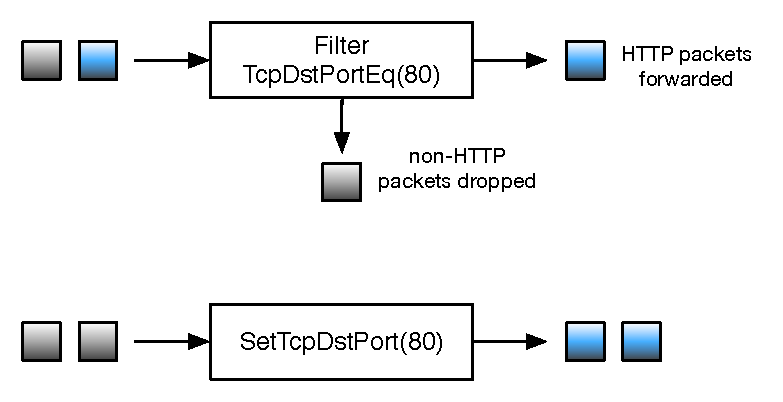
\includegraphics{netkat_policy_building_blocks}
\end{figure}

Here, the \texttt{TcpSrcPort} header gets
changed to 80.  This modification happens on a logical copy of the packet.  That means subsequent \texttt{Filters} 
match against the original \netkat{TcpSrcPort} 
value in the header, not the one we just changed it to.  But most of the 
time, you can ignore this subtlety because filters precede modifications.

Modifications to different headers can generally be specified in any order.  If two modifications to the same header 
value occur one after the other, the last one wins.  

You combine these building blocks with \texttt{Seq} and \texttt{Union}.
Here is a \texttt{Seq} of the two policies, a filter and a modification.   

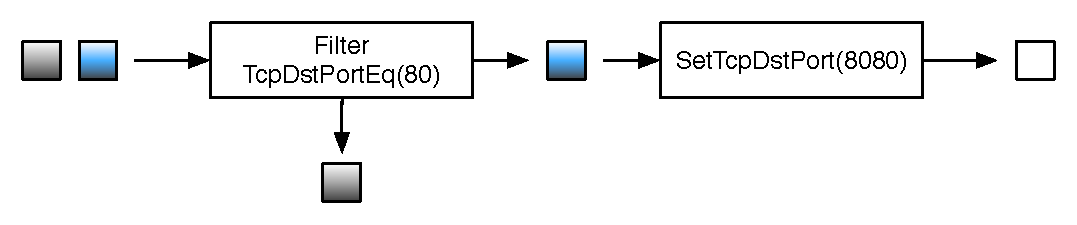
\includegraphics[width=\linewidth]{netkat_policy_combinators_seq}

In sequences, policies
are chained together in a straight line, and packets travel through each of one of the policies in order.  
Combining a filter plus modifications is very common in NetKAT programs, and we generally
use \texttt{Seq} to combine them into a \emph{rule}.  

A rule is like an OpenFlow flow table entry, but with more options.  
If you think about it, a switch receives a huge firehose blast of packets, and you want the switch to 
perform a targeted action on a very small subset of those packets. 
In other words, you want a \emph{filter} and some \emph{actions}.
It's like the MapReduce paradigm, but in reverse order - you first \emph{reduce} the stream to a manageable level,
then \emph{map} the result by performing actions on it.  

With \texttt{Seq}, order matters.  So the rule \texttt{drop >> Filter(EthTypeEq(0x806))} 
drops ALL packets, no matter the type.  
The second filter is never reached.  
In general, putting all the filters before the actions in a sequence chain is the clearest way to write it.

The following principle is a good guideline:  

\begin{principle}
Use \texttt{>>} between filters and all actions.
\end{principle}

For contrast let's look at \netkat{Union}.  Here is a \netkat{Union} of policies.

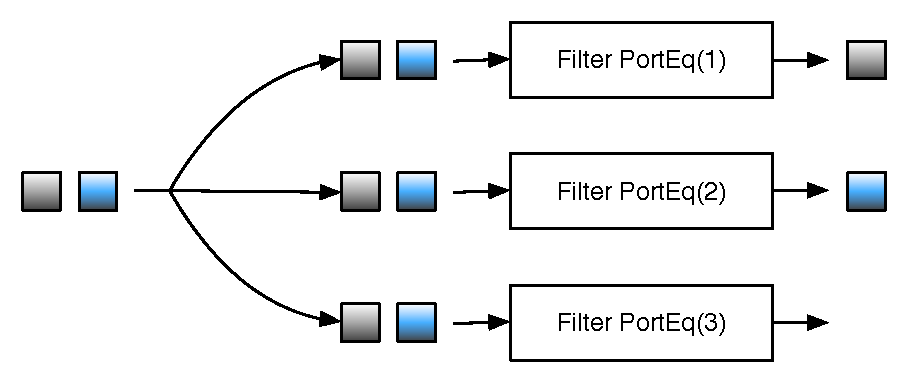
\includegraphics{netkat_policy_combinators_union}

A \texttt{Union} of policies makes logical copies of packets and sends the copy of each packet
through each policy in parallel.  In the above example, suppose the grey packet is from port 1 and the
blue packet is from port 2.  The two incoming packets are copied three times, one
for each rule.  In this case, the top filter only forwards a copy of the first packet matching \netkat{PortEq(1)}.
The middle filter only forwards a copy of the second packet  matching \netkat{PortEq(2)}
The bottom filter doesn't forward any packets at all.  

\begin{principle}
Use \texttt{|} between rules that DO NOT overlap.
Use \texttt{IfThenElse} to combine rules that DO overlap. 
\end{principle}

You might think, ``All that packet copying must be really tough on the switch.''  In fact, all the 
packet copying is conceptual, it doesn't necessarily happen in the switch.  Frenetic turns NetKAT
programs into flow tables, and these flow tables generally work through sophisticated TCAM's, Hash tables,
and pipelines that eliminate actual packet copying.  So don't worry about stringing 20,000 policies
with a \texttt{Union}.  Your switch can handle it.   

\texttt{SetPort} is a little different than other modifications.  
For example, \texttt{SetTcpDstPort} acts on a single packet at a time.
A single \texttt{SetPort} is like this - we merely want to change the egress port of the packet itself.  But if 
you want to send it out multiple ports at once, as in flooding, you can send a list of ports to \texttt{SetPort}.
It's equivalent to \netkat{Union}'ing a bunch of \netkat{SetPort} policies because you're copying the packet
to each port.  

Now let's look at \texttt{Union} and \texttt{IfThenElse}.  
As we have seen in Chapter 2, Union is parallel composition:
we effectively make copies of each packet and apply the rules to each packet.  So in our 
repeater application, the rules are:

\begin{itemize}
  \item \texttt{Filter(PortEq(1)) >> SetPort(2)} Sends traffic from port 1 out port 2 
  \item \texttt{Filter(PortEq(2)) >> SetPort(1)} Sends traffic from port 2 out port 1 
\end{itemize}

A packet cannot match both rules -- in other words, there is no overlap.  So a \texttt{Union} between
these two rules is appropriate.  You make a copy of each packet, send it through each of the rules.  
One or the other will match and send it out the appropriate port, the other will simply drop it.  

Suppose you have two rules:

\begin{itemize}
  \item \texttt{Filter(TcpDstPortEq(80)) >> drop} Drops non-encrypted HTTP traffic 
  \item \texttt{Filter(PortEq(2)) >> SetPort(1)} Sends port 2 traffic out port one.
\end{itemize}

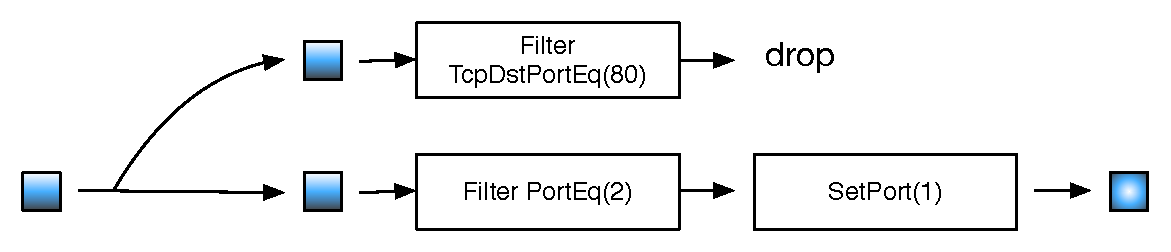
\includegraphics[width=\linewidth]{netkat_overlapping_union}

These two rules overlap.  A packet can both have a TCP destination port of 80 and
arrive on switch 1, port 2.  What happens if we combine them with \texttt{Union}, and a packet
like that arrives at the switch?  The packet will be copied twice, then:

\begin{itemize}
  \item \texttt{Filter(TcpDstPortEq(80)) >> drop} will drop the first copy of the packet 
  \item \texttt{Filter(PortEq(2)) >> SetPort(1)} will send out the second copy to port 1
\end{itemize}

But that's probably not what you intended.  You probably want the HTTP rule to take precedence over the
sending rule.  In such cases,
\texttt{IfThenElse} makes the precedence crystal clear:

\begin{minted}{python}
IfThenElse(TcpDstPortEq(80), drop, Filter(PortEq(2)) >> SetPort(1))}
\end{minted}

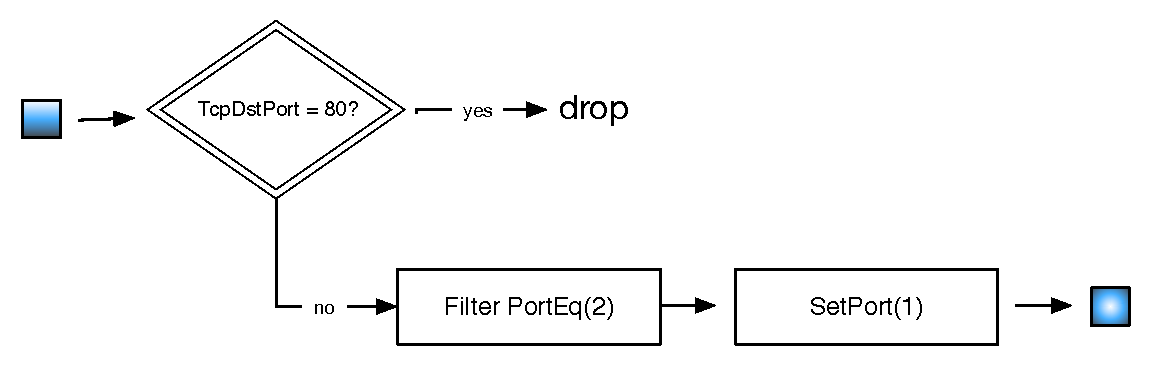
\includegraphics[width=\linewidth]{netkat_overlapping_if_then_else}

The predicate is tested, and if it matches, the first policy is performed, otherwise the second is performed.

That's pretty powerful, and in fact we can write the repeater app to use \texttt{IfThenElse} instead of Union:

\begin{minted}{python}
IfThenElse(PortEq(1), SetPort(2), Filter(PortEq(2)) >> SetPort(1) 
\end{minted}

So why not just use \texttt{IfThenElse} for combining rules all the time?  In a real switch, you might have 
hundreds of non-overlapping rules.  Writing them as:

\begin{minted}{python}
IfThenElse(predicate1), action1, IfThenElse(predicate2, action2, IfThenElse #....
\end{minted}

is doable but a lot more verbose.  It also hides the fact that the rules are non-overlapping, and this is useful
information when rummaging through an SDN app. 

\netkat{IfThenElse} is really syntactic sugar.  The statement:

\begin{minted}{python}
IfThenElse(pred, true_policy, false_policy)
\end{minted}

is just a shortcut for:

\begin{minted}{python}
Filter(pred) >> true_policy | Filter(~ pred) >> false_policy
\end{minted}

but it's a lot shorter and easier to understand, especially for programmers accustomed to seeing If-Then-Else
constructs in other programming languages.

\section{Keeping It Stateless}
\label{section:stateless}

So let's kick it up a notch.  
Our repeater is fast, but pretty static -- it only works with two ports, and only ports that are numbered
1 and 2.
So let's extend our repeater to do two things: 

\begin{enumerate}
\item On connection, read the list of currently available ports and build the initial NetKAT policy accordingly.
\item When ports go up or down, adjust the policy dynamically.
\end{enumerate}

The first task requires us to inquire which ports a switch has.  Frenetic provides a \texttt{current\_switches()}
method that does exactly that.   The best time to call it is on the \texttt{connected()} hook since, at that
point, Frenetic knows the switches and ports out there.

The following code is in \texttt{netkat\_principles/repeater3.py}:

\inputminted{python}{code/netkat_principles/repeater3.py}

\texttt{current\_switches()} is an asynchronous call, meaning you don't get the results immediately.
Instead, we pass a callback procedure named \texttt{handle\_current\_switches}, which Frenetic calls
when the \texttt{current\_switches()} call is complete and has results.  In our first pass, the callback
is just a one line procedure that prints the results to the log (the screen by default).  Although
we could define \texttt{handle\_current\_switches()} outside the \texttt{connected()} method, placing
it inside clarifies the connection between the two.  

So let's start up Mininet with 4 hosts this time:

\begin{minted}{console}
frenetic@ubuntu-1404:~/manual$ sudo mn --topo=single,4 --controller=remote
*** Creating network
*** Adding controller
Unable to contact the remote controller at 127.0.0.1:6633
*** Adding hosts:
h1 h2 h3 h4
*** Adding switches:
s1
*** Adding links:
(h1, s1) (h2, s1) (h3, s1) (h4, s1)
*** Configuring hosts
h1 h2 h3 h4
*** Starting controller
c0
*** Starting 1 switches
s1 ...
*** Starting CLI:
mininet>
\end{minted}

Start up Frenetic:

\begin{minted}{console}
frenetic@ubuntu-1404:~/manual$ frenetic http-controller --verbosity debug
 [INFO] Calling create!
 [INFO] Current uid: 1000
 [INFO] Successfully launched OpenFlow controller with pid 2035
 [INFO] Connecting to first OpenFlow server socket
 [INFO] Failed to open socket to OpenFlow server: (Unix.Unix_error "...
 [INFO] Retrying in 1 second
 [INFO] Successfully connected to first OpenFlow server socket
 [INFO] Connecting to second OpenFlow server socket
 [INFO] Successfully connected to second OpenFlow server socket
 [INFO] switch 1 connected
\end{minted}

And start up our application:

\begin{minted}{console}
frenetic@ubuntu-1404:~/manual/programmers_guide/code/principles$ python repeater3.py
No client_id specified. Using 0323e4bc31c94e81939d9f51640f1f5b
Starting the tornado event loop (does not return).
2016-04-12 09:51:14,578 [INFO] Connected to Frenetic - Switches: {1: [4, 2, 1, 3]}
\end{minted}

The \texttt{handle\_current\_switches} callback gets called with a Python dictionary.  
The keys in this dictionary are the datapath ID's (dpid's) of each switch -- in our case, we only have
one switch with a dpid of 1.
The value associated with the key is a list of ports that the switch has operational.  
In this case, we have four ports labelled 1 through 4 (they will be in some random order in the list, as
you see above in \python{[4, 2, 1, 3]}).

Great!  Once we have the list of ports, we can construct policies.  If a packet comes in on port
1, it should be repeated to all the ports that are not 1, e.g. 2, 3 and 4, and so on.   
The NetKAT policy, written out manually, will look like this:

\begin{minted}{python}
Filter(PortEq(1)) >> SetPort(2,3,4) |
Filter(PortEq(2)) >> SetPort(1,3,4) |
Filter(PortEq(3)) >> SetPort(1,2,4) |
Filter(PortEq(4)) >> SetPort(1,2,3)
\end{minted}

Or equivalently with lists:

\begin{minted}{python}
Filter(PortEq(1)) >> SetPort( [2,3,4] ) |
Filter(PortEq(2)) >> SetPort( [1,3,4] ) |
Filter(PortEq(3)) >> SetPort( [1,2,4] ) |
Filter(PortEq(4)) >> SetPort( [1,2,3] )
\end{minted}

A combination of Frenetic and Python lists makes this easy to construct.  
Suppose you have the list named \python{sw} with value 
\python{[1, 2, 3, 4]} from the callback.   The following Python list comprehension:

\begin{minted}{python}
[p for p in sw]
\end{minted}

returns the list \python{[1,2,3,4]}

Now suppose we're looking only at port 1.  We want all of the ports here 
except 1.  A little tweak to the list comprehension:

\begin{minted}{python}
[p for p in sw if p != in_port]
\end{minted}

Removes the input port from the list, leaving \python{[2,3,4]}

So here is our repeater that installs an initial configuration.
The following code is in \codefilename{netkat_principles/repeater4.py}:

\inputminted{python}{code/netkat_principles/repeater4.py}

Now it's just a hop, skip and  jump to a fully dynamic repeater.  First we need to capture packets from ports
that we haven't seen yet.  We could write an extremely long filter, filtering out every port that's not on the
list, but since port numbers can be 32-bits long, that's gonna be pretty huge:

\begin{minted}{python}
Filter(PortEq(5, 6, 7, ..., 4294967295) >> SendToController("repeater_app")
\end{minted}

It's easier just to write an overlapping rule.  Recall the \netkat{id} filter matches all packets:

\begin{minted}{python}
id >> SendToController("repeater_app")
\end{minted}

But obviously, this overlaps with the rules for known ports in our repeater.  So we use an \texttt{IfThenElse} to 
resolve the overlap:

\inputminted[firstline=14,lastline=25]{python}{code/netkat_principles/repeater5.py}

So if the port is a known port, we apply the \python{all_ports} policy.  Otherwise it's a known port
and we send the packet to the controller.

We take this opportunity to save the port list in an instance variable \texttt{self.all\_ports}.  This instance variable
is the beginning of a Network Information Base, or NIB -- it encapsulates the known state of the network
at this time.  We're going to see the NIB a lot in future apps.  You can think of our app as a function with the
NIB as input and a NetKAT program as output.  

Now how we do learn about new ports?  A packet arriving at \texttt{pkt\_in} will signal we're seeing a new port.
So suppose we're seeing a packet on port 40.  If you think about it, the entire NetKAT program will change from:

\begin{minted}{python}
Filter(PortEq(1)) >> SetPort(2,3,4) |
Filter(PortEq(2)) >> SetPort(1,3,4) |
Filter(PortEq(3)) >> SetPort(1,2,4) | 
Filter(PortEq(4)) >> SetPort(1,2,3)
\end{minted}

to:

\begin{minted}{python}
Filter(PortEq(1)) >> SetPort(2,3,4,40) |
Filter(PortEq(2)) >> SetPort(1,3,4,40) |
Filter(PortEq(3)) >> SetPort(1,2,4,40) | 
Filter(PortEq(4)) >> SetPort(1,2,3,40) |
Filter(PortEq(40)) >> SetPort(1,2,3,4)
\end{minted}

Fortunately, we have all the logic we need in \texttt{self.all\_ports\_policy} already.  We just need
to pass it an amended list of known ports.  Not a problem!

\begin{minted}{python}
  def packet_in(self, dpid, port_id, payload):
    self.all_ports.add(port_id)
    self.update(self.policy())
\end{minted}

What do we do with the packet we just received? 
We could just drop it and hope the host is smart enough to resend it.  But that's not
very hospitable.  

What if we just do a \texttt{pkt\_out} immediately afterward?  After all, we just installed a rule that
will deal with it appropriately, right?

\begin{minted}{python}
  def packet_in(self, dpid, port_id, payload):
    self.all_ports.add(port_id)
    self.update(self.policy())
    self.pkt_out(dpid, payload, ??? )
\end{minted}

There are two problems.  First, it's unclear what the action should be on \texttt{pkt\_out}.  If we send an empty 
list of actions, the OpenFlow switch will interpret it as ``drop the packet.''.  
Second, there's a timing problem.
Even though we just sent a self.update, the call is asynchronous with no response when it's done updating the
OpenFlow flow table.  It could take a microsecond, it could take an hour \ldots we just don't know.  
This timing problem actually can cause more problems.  What if, before the new rules are installed, the 
switch receives 100 more packets?  pkt\_in will be called 100 times, and each time the policy will
be recalculated and sent to the switch.  That could cause major problems since installing switch rules can
be a CPU-intensive process on the switch.

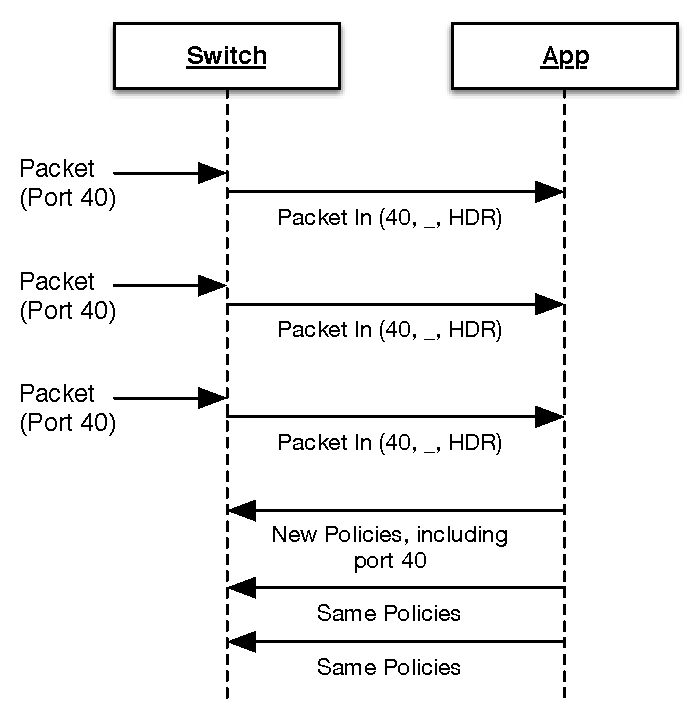
\includegraphics{netkat_policy_timing_problem}

Hence the following principle:

\begin{principle}
When you install a new switch policy, do not assume it'll be installed right away.  
\end{principle}

We can solve this with two quick fixes.  One is to make a quick check that port has not actually be learned yet.
The other is to add actions to pkt\_out that emulate the new rule.  

Here's our final repeater program in \codefilename{netkat_principles/repeater5.py}:

\inputminted{python}{code/netkat_principles/repeater5.py}

In mininet with a simple 4-host topology, we can test our repeater by adding a 5th host and port:

\begin{minted}{console}
mininet> py net.addHost('h5')
<Host h5:  pid=3187>
mininet> py net.addLink(s1, net.get('h5'))
<mininet.link.Link object at 0x7fd432ace810>
mininet> py s1.attach('s1-eth5')
mininet> py net.get('h5').cmd('ifconfig h5-eth0 10.5')
\end{minted}

The new port causes the switch to send an OpenFlow portUp message to our app.  We don't have a handler for
the \texttt{port\_up} hook, so the default message appears:

\begin{minted}{python}
port_up(switch_id=1, port_id=5)
\end{minted}

Back in Mininet, let's try to ping from our new host:

\begin{minted}{console}
mininet> h5 ping -c 1 h1
PING 10.0.0.1 (10.0.0.1) 56(84) bytes of data.
64 bytes from 10.0.0.1: icmp_seq=1 ttl=64 time=996 ms

--- 10.0.0.1 ping statistics ---
1 packets transmitted, 1 received, 0% packet loss, time 0ms
rtt min/avg/max/mdev = 996.738/996.738/996.738/0.000 ms
\end{minted}

Looks good!  A combination of the new packet rules and the \texttt{pkt\_out} 
is sending the packets to the correct place.  

\section{Summary}

In building a dynamic repeater, we have learned the following NetKAT principles:

\setcounter{principle}{0}

\begin{principle}
Keep as much traffic out of the controller as possible.
Instead, program NetKAT policies to make most of the decisions inside the switch.  
\end{principle}

\begin{principle}
Use \texttt{>>} between filters and all actions.
\end{principle}

\begin{principle}
Use \texttt{|} between rules that DO NOT overlap.
Use \texttt{IfThenElse} to combine rules that DO overlap. 
\end{principle}

\begin{principle}
When you install a new switch policy, do not assume it'll be installed right away.  
\end{principle}

And we'll learn a fifth in the next chapter:

\begin{principle}
Do not rely on network state.  Always assume the current packet is the first one you're seeing.   
\end{principle}

These principles are meant as guidelines, not straitjackets.
As we build network applications over the next few chapters, we may find good reasons to violate them 
to achieve shorter code or better modularity.
That's OK. 

Now we have a robust repeater that acts mostly correctly.  There is a still a small timing problem.  If a packet
arrives from port 1 bound for port 40 in that short interval before the rules for port 40 are installed, it
will be copied to ports 2, 3, and 4 but not 40.  There's little we can do in the context of our simple repeater.

But of course, modern network equipment doesn't act like a repeater.  That's 1980's technology!  Repeaters
do a lot of unnecessary packet copying, flooding hosts with packets that are clearly destined for them.  
So our next project will be building an L2 learning switch.  In that context, we'll correct some of the 
remaining timing flaws.  And the result will be much more efficient. 


% !TEX root = frenetic_programmers_guide.tex

\chapter{Learning Switch}

\section{Design}
\label{l2_learning_switch:design}

Layer 2, or L2, switching revolutionized networking in the 1990's.
As LAN traffic grew, hub performance rapidly degraded as collisions became more and more frequent.
L2 switches effectively cut the LAN into logical segments, performing the forwarding between them.
This dramatically reduced the number of collisions, and also cut down on the traffic that individual
NIC's had to filter out.  Just as the Plain Old 
Telephone System evolved from party lines to direct lines, LAN hardware evolved from Hubs to 
L2 switches, improving security, speed and signal quality.

Of course, L2 switches were more technically sophisticated than hubs.  They required a processor, memory, and 
some form of software.  In order to know which segments to forward traffic, they needed to 
watch the Ethernet MAC addresses of traffic and theremember their respective ports.  In other words, the switch 
\emph{learns} the MAC-to-port mappings, and thus L2 switches are called learning switches.    

We can simulate the L2 switch with Frenetic.  By doing so, as well see in 
Section \ref{l2_learning_switch:timeouts},
we can add features to the switch with just a little extra programming effort.  At a high-level, 
you can think of a Frenetic network application as:

$$ netkat = f( nib, env ) $$

Where $f$ is your application, $nib$ is the Network Information Base -- the information you have dynamically determined in your network through
packets received by \netkat{pkt_in} -- and
$env$ is other information (fixed configuration files, out-of-band network measurements, or whatever you want).  
The output, $netkat$ is the NetKAT program.

Naturally, $nib$ is critical to a good design.  You don't need to capture all aspects of the network,
only those needed to properly form switch rules.  In an L2 switch, we are really only interested in three 
pieces of data in a packet:

\begin{itemize}
\item The source MAC address
\item The destination MAC address
\item The switch port connected to the host with a particular MAC address
\end{itemize}

So that's all the data we want to capture for the NIB.  Here's a rough design for how we want the switch to behave:

\begin{minted}{python}
if port_for_mac(EthSrc) == None:
  learn(EthSrc, Port)
if port_for_mac(EthDst) != None:
  pkt_out(payload, port)
else
  pkt_out(payload, all_ports_except(port))
\end{minted}

Admittedly this is pretty sketchy, but it covers the interesting cases.  In particular, it covers
Ethernet broadcasts to MAC address ff:ff:ff:ff:ff:ff just by the fact that a source MAC will never
equal ff:ff:ff:ff:ff:ff.  And flooding is exactly what you want to do in that case.

So our NIB must maintain at least a list of MAC-to-port mappings.  
In our Repeater app, our NIB was a single instance variable in the application itself:
\netkat{self.ports}, which held a list of connected ports on the switch.  
Now we'll evolve a little.
In what will become a standard
part of our network apps, we'll model the NIB as a separate object class in Python.  
The following code is in \codefilename{l2_learning_switch/network_information_base.py}:

\inputminted{python}{code/l2_learning_switch/network_information_base.py}

That 
encapsulates the state in one place, making it easy to change underlying data structures later.
It also separates the NIB details from the NetKAT details, making it easier to reuse the NIB
in other applications.  

\section{A First Pass}

One of the problems with our switch pseudocode design is it doesn't fit our notions of NetKAT very well.
NetKAT programs do not have variables, so they can't remember MAC-to-port mappings on their own.
So it appears that every packet must pass through the controller so we can make decisions.
Processing every single packet through the controller clearly violates the First NetKAT principle, but
we can leave that aside for now.  It'll be instructive to build an easy but inefficient L2 switch first.

The following code is in \codefilename{l2_learning_switch/learning1.py}:

\inputminted[linenos]{python}{code/l2_learning_switch/learning1.py}

There are a couple of new details to note:

\begin{itemize}
\item The \netkat{__init__} constructor must call the superclass constructor to properly initialize.
\item Because we are writing in classes, we now distinguish the main loop of this application with 
a check on \netkat{__main__}.  
\item We are using the Frenetic \python{Packet} object discussed in Section \ref{introduction:packet_in}
\item The \netkat{packet_in} looks almost exactly like our pseudocode design
\end{itemize}

Starting up Mininet, Frenetic and our application respectively, we try a \netkat{pingall} in Mininet and see
the following on the console:

\begin{minted}{console}
frenetic@ubuntu-1404:~/manual/programmers_guide/code/l2_learning_switch$ python learning1.py
Starting the tornado event loop (does not return).
2016-04-14 12:49:17,228 [INFO] Connected to Frenetic - Switches: {1: [4, 2, 1, 3]}
2016-04-14 12:49:17,229 [INFO] Learning: 9a:0f:ec:39:54:f5 attached to ( 1 )
2016-04-14 12:49:17,258 [INFO] Learning: be:3f:5a:90:8a:ac attached to ( 2 )
2016-04-14 12:49:17,303 [INFO] Learning: 3a:a4:6b:e6:24:25 attached to ( 3 )
2016-04-14 12:49:17,343 [INFO] Learning: f2:a7:c0:cb:90:23 attached to ( 4 )
\end{minted}

The switch works perfectly!  But it's a huge violation of Principle 1: all the traffic 
goes through the controller.  

\section{A More Efficient Switch}

Once we've learned a MAC-to-port
mapping, we shouldn't have to go to the controller for packets destined for that MAC.  The switch
should handle it by itself.

This is actually pretty straightforward.  If we know that MAC 11:11:11:11:11:11 is on port 2, we
can handle it with the following NetKAT program:

\begin{minted}{python}
Filter(EthDstEq("11:11:11:11:11:11")) >> SetPort(2)
\end{minted}

And we just need one of these rules for each MAC we've learned.  But all of these rules are non-overlapping
because they involve different values for \netkat{EthDst}.  So we just Union them all together and that's
our entire NetKAT program.

So let's write some methods for calculating the policies
We'll add this code to learning1 (listed in \codefilename{l2_learning_switch/learning2.py}):

\inputminted[firstline=23,lastline=31]{python}{code/l2_learning_switch/learning2.py}

Note here that \python{(mac, port) = mac_port} unpacks the tuple \python{mac_port} into two variables
\python{mac} and \python{port}.

When shall we install these rules?   We could install them on every incoming packet, but that's a little
overkill. We really only need to recalculate them when we see a newly learned MAC and port.  So we add them
to that conditional:

\inputminted[firstline=41,lastline=43]{python}{code/l2_learning_switch/learning2.py}

Now run it and try a pingall from Mininet:

\begin{minted}{console}
frenetic@ubuntu-1404:~/manual/programmers_guide/code/l2_learning_switch$ python learning1.py
Starting the tornado event loop (does not return).
2016-04-14 13:33:22,965 [INFO] Connected to Frenetic - Switches: {1: [2, 4, 1, 3]}
2016-04-14 13:33:26,447 [INFO] Learning: 86:d8:df:f0:95:75 attached to ( 1 )
2016-04-14 13:33:26,453 [INFO] Learning: 4a:1c:9e:9b:50:7c attached to ( 2 )
... STOP
\end{minted}

Uh oh.  Why did we only learn the first two ports?   Let's look at the Frenetic console for a clue:

\begin{minted}{console}
[DEBUG] Installing policy
drop |
(filter ethDst = 4a:1c:9e:9b:50:7c; port := 2 |
 filter ethDst = 86:d8:df:f0:95:75; port := 1)
[DEBUG] Setting up flow table
+----------------------------------------+
| 1 | Pattern                | Action    |
|----------------------------------------|
| EthDst = 4a:1c:9e:9b:50:7c | Output(2) |
|----------------------------------------|
| EthDst = 86:d8:df:f0:95:75 | Output(1) |
|----------------------------------------|
|                            |           |
+----------------------------------------+
\end{minted}

Can you see the problem?  There's no longer a rule to send packets to the controller.  If packets
are destined for the first two MAC addresses, that's not a problem.  But if they're destined for
other MAC addresses, it \emph{is} a problem.

If that's true, why didn't it stop after the first packet?  Remember NetKAT Principle 4, which 
states there is a lag time between rule sending and rule installation.  In this case:

\begin{enumerate}
\item The first packet came to the controller, causing a rule regeneration.  These rules
are sent to the switch, but are not installed yet.
\item The second packet came to the controller, causing a second rule regeneration.
\item The rules from the first packet are installed on the switch, effectively shutting off 
any more packets from going to the controller.
\item The rules from the second packet are installed.  
\end{enumerate}

One thing that definitely \emph{won't} work is to add the following rule with a Union:

\begin{minted}{python}
id >> SendToController("learning_app")
\end{minted}

The \netkat{id} filter matches all packets, and therefore overlaps every other rule.  Even if we place this
rule as the last rule in a set of Unions, \emph{that does not guarantee it'll be fired last.}  Frenetic 
does not guarantee the OpenFlow rules will follow the order of the NetKAT rules.     

There are a few ways to solve this problem, but we'll try an easy one first.  
In Chapter 2, we mentioned briefly that for every \netkat{FieldEq} NetKAT predicate, there is a corresponding
\netkat{FieldNotEq} predicate.  We can use that in our policy, as we see in \netkat{learning3.py}:

\inputminted[firstline=30,lastline=37]{python}{code/l2_learning_switch/learning3.py}

Basically, we want to see all packets with an unfamiliar Ethernet source MAC (because we want to learn the
port) or destination MAC (because we need to flood it out all ports).  Although we could set up 
NetKAT policies to handle the latter case, it tends to be overkill since an unlearned destination MAC
usually replies soon afterwards, the MAC is learned, and everything is good.  

Notice how the this fairly simple NetKAT policy becomes a large OpenFlow table:

\begin{minted}{console}
[DEBUG] Setting up flow table
+------------------------------------------------------+
| 1 | Pattern                | Action                  |
|------------------------------------------------------|
| EthDst = 00:00:00:00:00:01 | Output(1)               |
| EthSrc = 00:00:00:00:00:01 |                         |
|------------------------------------------------------|
| EthDst = 00:00:00:00:00:01 | Output(1)               |
| EthSrc = 00:00:00:00:00:02 |                         |
|------------------------------------------------------|
| EthDst = 00:00:00:00:00:01 | Output(1)               |
| EthSrc = 00:00:00:00:00:03 |                         |
|------------------------------------------------------|
| EthDst = 00:00:00:00:00:01 | Output(1)               |
| EthSrc = 00:00:00:00:00:04 |                         |
|------------------------------------------------------|
| EthDst = 00:00:00:00:00:01 | Output(Controller(128)) |
|------------------------------------------------------|
...
\end{minted}

In fact, the table will have $n^2$ entries where $n$ is the number of learned MACs.  It's a lot easier
to write the NetKAT rules than all these OpenFlow rules.  

\section{Timeouts and Port Moves}
\label{l2_learning_switch:timeouts}

Our learning switch works fine if MAC-to-port assignments never change.  But a network is usually
more fluid than that:

\begin{itemize}
\item Users unplug a host from one port and plug it into another.  In our application, packets will
continue to go to the old port.
\item Users replace one host (and associated MAC) with another host in the same port.  In our application, the
old MAC will continue to take up rule space on the switch, making it more confusing to debug. 
\end{itemize}

Fortunately, plugging and unplugging hosts sends OpenFlow events \netkat{port_up} and \netkat{port_down},
respectively.  We can write hooks that control MAC learning and unlearning.  The following
code is in \netkat{learning4.py}:

\inputminted[firstline=65,lastline=74]{python}{code/l2_learning_switch/learning4.py}

When we make a port change, we call \netkat{update()} to recalculate and send the NetKAT rules down to the 
switch.  This keeps the forwarding tables in sync with the NIB.  

If we can rely on \netkat{port_up} and \netkat{port_down} events, this approach would work fine.
However, in the real world, the following things can happen:

\begin{itemize}
\item The \netkat{port_up} or \netkat{port_down} message might not fire.  Since they rely on power being
present or absent, they are not always reliable.
\item The messages might arrive in the wrong order, as in the port ``flip-flopping'' between active and 
inactive status.
\end{itemize}

Modern switches solve these issues by holding MAC-to-port mappings for a certain amount of time, then 
timing them out and (if they're still connected) relearning them.  Pure OpenFlow flow rules emulate
this by assigning a timeout value to each flow rule.   But NetKAT doesn't have timeouts, and indeed since
NetKAT policies don't map one-to-one to flow table rules, it'd be difficult to pass this information on.

But our application obeys the following principle:

\setcounter{principle}{4}

\begin{principle}
Do not rely on network state.  Always assume the current packet is the first one you're seeing.   
\end{principle}
 
That means we can restart the application at any time.  This clears out the NIB and sets the flow table
back to its initial ``send all packets to controller'' state.  
There will be a slight performance penalty as MAC-to-port mappings are relearned, but eventually the
NIB will be filled wth all current MAC addresses \ldots and no outdated ones.

Following this principle yields another benefit: fault tolerance.  If the switch loses connectivity with 
our application, the switch will continue to function.  No new MACs will be learned, but otherwise the 
network will continue to run.  When the application returns, it will start with a clear NIB and relearn MACs.  

In other words, a fully populated NIB is not critical to switch operation.  It makes things much faster
by providing the basis for the NetKAT rules.  But it's not so important that it needs to be persisted or
shared, making the overall design much simpler.  

\section{Summary}

Our learning switch application is a mere 130 lines of code, but it does a lot:

\begin{itemize}
\item Mac addresses are learned in the NIB as packets arrive at the switch
\item The flow table is updated to match the NIB
\item Broadcast packets are automatically forwarded to all ports
\item It handles hosts moved to other ports or replaced with other devices
\item It is fault tolerant, and can easily tolerate restarts
\end{itemize}

The latest traditional switches can do even more.  For example, you can plugin a Wireless Access Port or 
WAP to a switch port.  Practically, the WAP acts like a multiplexer allowing multiple MACs to 
attach to a single port.   It turns out our application handle multiple MACs mapped to a port, although it's 
difficult to model this in Mininet.  We can enforce certain security constraints, like the number of MACs on
a particular WAP, simply by changing the NIB class.

It's this kind of flexibility that makes SDN an important evolutionary move.  In the next chapter, we'll
inject some more intelligence into the network to handle Virtual LANs, or VLANs. 
\chapter{Proxy ARP}

\section{The ARP Protocol}
 \label{proxy_arp:protocol}

\section{Design}

\section{Snooping on ARP Requests and Replies}

\section{Replying}

\section{Maintaining State Across Restarts}


% !TEX root = frenetic_programmers_guide.tex

\chapter{Handling VLANs}

\section{VLAN Uses}
\label{handling_vlans:uses}

Back in the late 1990's when LAN switching became more prevalent, network architects ran into balancing problems.
Enterprise divisions and departments wanted to keep their 
LANs separate for security and speed reasons.  For example, departments that generated heavy traffic 
during certain times of the month (like the Accounting department) needed to be segregated from others
to prevent intolerable slowdowns in other departments.  

The problem was network boundaries had to match physical switch boundaries.  If you bought switches with
48 ports, and a department had 12 hosts, then 36 would remain unused.  Worse, if a department grew from 
48 to to 49 ports, you had to make an emergency network buy.  

Networks often solved these problems by adding routers, splitting department subnets and letting the 
routers handle traffic between them.  But routing can be expensive and slow, especially for large 
bursts of traffic.  Routing makes sense between networks you want to keep segregated, but it's
overkill between two hosts that you know you want to keep together.

Virtual LAN's, called VLAN's, emerged to solve these problems.  You can think of a VLAN as a logical 
network, mappable onto physical switches.  A VLAN is like an elastic switch -- you assign real ports to 
a particular VLAN, then can add or remove them at will.  

VLANs can span multiple switches.  So if you needed that 49th port for a department, you could assign 
an unused port on a different switch to that VLAN, and the host on it would act as if it were connected to 
the same switch.  Of course, there's technically more to it than that, especially since you need to get the
packet from one switch to the other.  But as a network operator, VLANs freed you from worrying about
those details.  

OpenFlow-based switches and Frenetic can integrate with standard VLAN technology easily.  In this 
chapter, we'll first simulate a simple VLAN in software.  Then we'll use standard 802.1Q VLANs to 
make a more flexible setup.  Then we'll use VLAN technology between switches.  

\section{A Simple, Fixed VLAN}

You've probably noticed that, as we're designing networking applications we start with something 
static and hard-coded, then gradually move to something configurable and dynamic.  This kind of 
organic growth makes network application design more agile.
It's easier to start with a simple net app, debug it, then add and test more functionality a bit at a time.  

So we'll start with a simple rule-based VLAN structure:

\begin{itemize}
\item Odd-numbered ports (1, 3, 5, \ldots) will get mapped to VLAN 1001
\item Even-numbered ports (2, 4, 6, \ldots) will get mapped to VLAN 1002
\end{itemize}

The VLAN ids 1001 and 1002 will only be used internally for this first application.  Later, we'll use
them as actual 802.1Q VLAN ids, since they fit into the range 1..4096.  

Hosts in each VLAN will talk only to hosts in their own VLAN, never to hosts in the other VLAN.  We'll talk
about how to connect the two VLANs together a little later.  

As we saw in Chapter 4, in NetKAT the L2 switch basic rule looks like this:

\begin{minted}{python}
Filter(EthDstEq("11:11:11:11:11:11")) >> SetPort(2)
\end{minted}

In our new VLAN-based network, port 2 is on VLAN 1002, to which all even-numbered ports belong.  
To segregate the networks, we'll simply extend the rule to look like this:

\begin{minted}{python}
Filter(PortEq(2,4,6,8,10)) >> Filter(EthDstEq("11:11:11:11:11:11")) >> SetPort(2)
\end{minted}

Where we cobble together $2, 4, 6\ldots$ from the even-numbered ports we know about on the switch.  

If the destination is unknown, instead of flooding packets out \emph{all} ports of the switch, 
we'll flood over ports of the switch \emph{in the same VLAN}.  In other words, the Packet Out action 
for a packet arriving at port 4 will be:

\begin{minted}{python}
SetPort(2,6,8,10)
\end{minted}

We'll add some methods onto the \python{NetworkInformationBase} object to do some VLAN mapping.  The following
code is in \codefilename{code/handling_vlans/network_information_base_static.py}:

\inputminted[firstline=60]{python}{code/handling_vlans/network_information_base_static.py}

The \python{policy_for_dest} method gets extended with the new filtering.  
The following
code is in \codefilename{code/handling_vlans/vlan1.py}:

\inputminted[firstline=23,lastline=30]{python}{code/handling_vlans/vlan1.py}

And the \python{packet_in} handler does some extra VLAN handling.  Note that if the destination port is already
learned, we verify it's connected to the same VLAN as the source.  That way, hosts cannot just forge 
destination MAC addresses in the other VLAN and subvert security.  

\inputminted[firstline=43,lastline=73]{python}{code/handling_vlans/vlan1.py}

Otherwise, learning switch internals stay the same.  Using a \python{single,4} topology in Mininet,
a pingall:

\begin{minted}{console}
mininet> pingall
*** Ping: testing ping reachability
h1 -> X h3 X
h2 -> X X h4
h3 -> h1 X X
h4 -> X h2 X
*** Results: 66\% dropped (4/12 received)
mininet>
\end{minted}

reveals that only odd-numbered ports talk to odd-numbered ports, and only even-numbered ports talk to
even-numbered ports.  We now have two segregated VLANs.

\section{Standard, Dynamic VLANs}

So now we want to make our setup a little more flexible.  Our program effectively codes the port-to-VLAN
mappings.  We \emph{could} also store this mapping in a configuration file or a database.  But even that's
too static.  We want network operators to be able to change VLAN-to-port mappings on the fly, simply
by changing the interface configuration on the switch.

So how are VLANs assigned to ports?  The procedure varies from switch to switch, but in most cases you
create an \emph{untagged} interface.  On an HP switch, for example, you configure the interface information
like this:

\begin{minted}{console}
coscintest-sw-ithaca# config
coscintest-sw-ithaca(vlan-1)# vlan 1001
coscintest-sw-ithaca(vlan-1001)# untagged A1
\end{minted}

This assigns the port A1 to VLAN 1001.  On OpenVSwitch, which is the OpenFlow switch we're using under Mininet, 
the configuration is similar:

\begin{quotation}
\emph{NOTE: The following tag setting commands don't seem to work correctly on the OpenVSwitch version found on
Frenetic VM.  Packet In messages have no VLAN tag.  One nasty workaround is to use a custom Mininet 
topology, where a separate driver attached to an IP address on each Mininet host sends VLAN-tagged packets.
This is not only a pain to model, but it's not how real OpenFlow switches (like the Dell and HP) handle
VLANs.  }
\end{quotation}

\begin{minted}{console}
mininet> sh ovs-vsctl set port s1-eth1 tag=1001
mininet> sh ovs-vsctl set port s1-eth2 tag=1002
mininet> sh ovs-vsctl set port s1-eth3 tag=1001
mininet> sh ovs-vsctl set port s1-eth4 tag=1002
mininet> sh ovs-vsctl show
ae82ea91-2820-4b9f-9b01-fd8e897675b9
    Bridge "s1"
        Controller "tcp:127.0.0.1:6633"
        Controller "ptcp:6634"
        fail_mode: secure
        Port "s1-eth4"
            tag: 1002
            Interface "s1-eth4"
        Port "s1"
            Interface "s1"
                type: internal
        Port "s1-eth2"
            tag: 1002
            Interface "s1-eth2"
        Port "s1-eth1"
            tag: 1001
            Interface "s1-eth1"
        Port "s1-eth3"
            tag: 1001
            Interface "s1-eth3"
    ovs_version: "2.1.3"
\end{minted}

That means any packets going into this port without any VLAN
information (i.e. untagged) are implicitly tagged with a fixed VLAN id.   This VLAN id is visible in NetKAT
predicates, and in the \python{packet_in} hook, even though they technically don't belong to the 
packet that entered the switch.  (This is a rare instance where packet modifications are applied
before Frenetic gets ahold of them.)

Outgoing packets on these ports have VLAN information stripped from them.  That's because we generally 
want hosts to be unencumbered by VLAN information.  This allows us to move the host from one VLAN to another
without reconfiguring the host itself.  

In our net app, learning VLAN-to-port mappings is very similar to learning MAC-to-port mappings.  In fact, 
we can do it all at the
same time.  We assume that an incoming packet for port $p$ with a VLAN tag of $v$ can be learned as a 
VLAN-to-port mapping.  If a port is ever reassigned to another VLAN, the same \python{port_down} and
\python{port_up} hooks will be fired as for MAC moves, so we can unlearn the VLAN mappings at the same
time.  

We'll store the VLAN-to-port mappings in a Python dictionary, similar to our MAC-to-port mappings.  
One difference is the values of this dictionary will be lists, since a VLAN (the key of our dictionary)
will be assigned to many ports.  This code will will replace our static VLAN view in 
\codefilename{code/handling_vlans/network_information_base_static.py}:

\inputminted[firstline=65]{python}{code/handling_vlans/network_information_base_dynamic.py}

Then we tweak the \python{learn} method to learn both MACs and VLANs:

\inputminted[firstline=13,lastline=24]{python}{code/handling_vlans/network_information_base_dynamic.py}

And in the \python{delete_port} method, we clean up any lingering VLAN-to-port mappings for that port:

\inputminted[firstline=55,lastline=60]{python}{code/handling_vlans/network_information_base_dynamic.py}

Since we now have packets tagged with VLANs, the NetKAT policies no longer need to reference list of ports.
They will change to look like:

\begin{minted}{python}
Filter(VlanEq(1002)) >> Filter(EthDstEq("11:11:11:11:11:11")) >> SetPort(2)
\end{minted}

Which we enshrine in the \python{policy_for_dest} method, listed in 
\codefilename{code/handling_vlans/vlan2.py}:

\inputminted[firstline=23,lastline=29]{python}{code/handling_vlans/vlan2.py}

In the \python{packet_in} handler, we read the VLAN from the packet instead of precomputing it:

\inputminted[firstline=42,lastline=71]{python}{code/handling_vlans/vlan2.py}

And now our switch handles VLANs dynamically.  You can create new VLANs, assign ports to them, rearrange or
dismantle them altogether, all without restarting the network application.  

\section{Summary}

Virtual LANs, or VLANs, introduce a level of indirection in creating a network.  Before them, physical
switches forced physical boundaries on the design.  Overprovisioning meant that many switches had
unused ports while other switches were filled to the brim.  

In this chapter we created:

\begin{itemize}
\item An application that simulates VLANs algorithmically
\item And an extended, dynamic application that reads VLAN information from packets and adjust accordingly, 
similar to our learning switch.
\end{itemize}

Note that you can combine these two approaches.  You can enforce certain rules, such as "ports 1-35 will always
be access ports assigned to VLANs 1000-1999, ports 35 and up will be on the management VLAN 1."  This is an
excellent use case for SDN -- your rules will never be hampered by an inflexible switch.

Up until this point, we have been working with one switch, which makes things easy to design.  But multiple
switches will extend the range of our network greatly.  They come with their own sets of challenges though,
which we'll work through in our next chapter.  
% !TEX root = frenetic_programmers_guide.tex

\chapter{Gathering Statistics}
\label{chapter:statistics}

\section{Port Statistics}

Frenetic has two statistics-gathering mechanisms:

\begin{itemize}
\item The \netkat{port_stats} command gets per-port statistics.
\item The \netkat{SetQuery} policy gathers user-defined statistics.  You can use this in switch
policies or \netkat{pkt_out} actions, and aggregate them.
\end{itemize}

\begin{quotation}
\emph{SetQuery is not in the current Python bindings, but will be.  See Issue \#491 on Github}
\end{quotation}

We could add the statistics-gathering commands to an existing network application, like our learning
switch.  But Frenetic allows you more flexibility.   

We're going to write a completely separate application and run it as a separate process, but point it
at the same Frenetic instance as the learning switch.  The architecture looks something like this:

\begin{figure}[h]
\centering
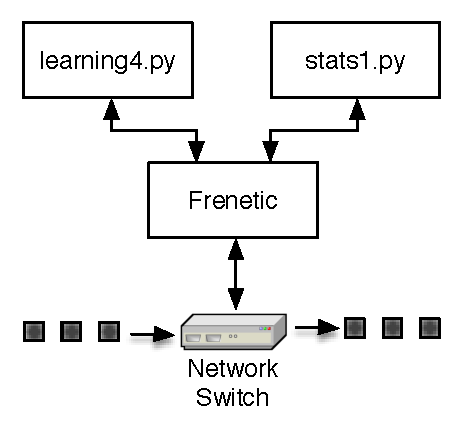
\includegraphics{dual_app_frenetic_architecture}
\end{figure}

This yields some nice advantages:

\begin{itemize}
\item We can combine the statistics application with other network applications.  It's like a 
library of network functions.
\item The resulting applications are much smaller, focused, and easy to understand and debug.
\item If the applications have large NetKAT policies, the process of separating them makes the 
updating them a bit faster.
\item If the applications are CPU intensive, you can run them on different servers or in different VM's.
\end{itemize}

One caveat is that all NetKAT policies from the applications are \netkat{Union}'ed together.  
Therefore, according
to NetKAT Principle 3, they should not have overlapping rules.  If this is a problem, you can use 
concerns to modularize your application instead, which we'll cover in Chapter \ref{chapter:modularization}.

The NIB for our statistics gathering process is fairly simple -- we save just the switch DPID and 
port list.  Although we could share the NIB with the other applications, keeping it separate frees us
from worrying about locks and so forth

The following code is in \codefilename{gathering_statistics/network_information_base.py}:

\inputminted{python}{code/gathering_statistics/network_information_base.py}

The statistics program itself doesn't need to send any NetKAT policies.  We set a 5 second timer,
and send the \netkat{port_stats} command each time, logging the response:

The following code is in \codefilename{gathering_statistics/stats1.py}:

\inputminted{python}{code/gathering_statistics/stats1.py}

Having started Mininet, Frenetic, and the Learning switch \codefilename{learning4.py} from Section 
\ref{l2_learning_switch:timeouts}, we can now start our app independently:

\begin{minted}{console}
vagrant@frenetic:~/manual/programmers_guide/code/gathering_statistics$ python stats1.py
Starting the tornado event loop (does not return).
2016-04-29 10:33:37,321 [INFO] Connected to Frenetic - Switches: {1: [4, 2, 1, 3]}
2016-04-29 10:33:42,333 [INFO] Count 1@3: {rx_bytes = 9590, tx_bytes = 10206}
2016-04-29 10:33:42,333 [INFO] Count 1@4: {rx_bytes = 8414, tx_bytes = 9100}
2016-04-29 10:33:42,334 [INFO] Count 1@2: {rx_bytes = 9562, tx_bytes = 10276}
2016-04-29 10:33:42,334 [INFO] Count 1@1: {rx_bytes = 10024, tx_bytes = 9184}
\end{minted}

Doing a \texttt{pingall} in the Mininet window will make the statistics go up.

What per-port statistics are available?  The following table gives you a list:

\begin{description}
\item[port\_no] Port number  
\item[rx\_packets] Number of packets received  
\item[tx\_packets] Number of packets transmitted  
\item[rx\_bytes] Number of bytes received  
\item[tx\_bytes] Number of bytes transmitted  
\item[rx\_dropped] Number of packets attempted to receive, but dropped  
\item[tx\_dropped] Number of packets attempted to transmit, but dropped
\item[rx\_errors] Number of packets errored upon receive 
\item[tx\_errors] Number of packets errored upon transmit
\item[rx\_fram\_err] Number of packets received with frame errors
\item[rx\_over\_err] Number of packets received with buffer overrun errors
\item[rx\_crc\_err] Number of packets received with CRC errors
\item[collisions] Number of collisions detected
\end{description}

These are the per-port statistics defined in OpenFlow 1.0.  

\section{Queries}
\label{statistics:queries}

You can also gather statistics based on NetKAT rules.  This is called a \emph{query} and you can think 
of a query as just another location to send packets, like \netkat{SetPort} or \netkat{SetPipe}.
So Principle TODO applies here.  Recall that a packet can have only one destination: a port, a pipe or a 
query.  If you want packets to go to more than one destination, you need to use \netkat{Union} between
them so packet copies are made.

Unlike per-port statistics, a query only counts two things:

\begin{description}
\item[0] Number of packets  
\item[1] Number of bytes  
\end{description}

You call the \python{self.query()} command to get the current counts for this query at any time.

The following code is in \codefilename{gathering_statistics/stats2.py}:

\inputminted{python}{code/gathering_statistics/stats2.py}

So here, we set up a query called \python{"http"} and use it as a location to send packets.  The rule 
counts only HTTP requests initiated from port 1.  Every five minutes, we ask for a current count
from the query.  We can simulate an HTTP in Mininet like this:

\begin{minted}{console}
vagrant@frenetic:~$ sudo mn --topo=single,2 --controller=remote --mac
*** Creating network
*** Adding controller
Unable to contact the remote controller at 127.0.0.1:6633
*** Adding hosts:
h1 h2
*** Adding switches:
s1
*** Adding links:
(h1, s1) (h2, s1)
*** Configuring hosts
h1 h2
*** Starting controller
c0
*** Starting 1 switches
s1 ...
*** Starting CLI:
mininet> h2 python -m SimpleHTTPServer 80 &
mininet> h1 curl 10.0.0.2
<!DOCTYPE html PUBLIC "-//W3C//DTD HTML 3.2 Final//EN"><html>

 ... More output 
\end{minted}

And the output changes when the request is initiated:

\begin{minted}{console}
Starting the tornado event loop (does not return).
2016-05-11 14:51:46,565 [INFO] Connected to Frenetic - Switches: {1: [2, 4, 1, 3]}
2016-05-11 14:52:06,572 [INFO] Count: {packets = 0, bytes = 0}
2016-05-11 14:52:11,571 [INFO] Count: {packets = 0, bytes = 0}
2016-05-11 14:58:18,802 [INFO] Count: {packets = 11, bytes = 806}
2016-05-11 14:58:23,802 [INFO] Count: {packets = 11, bytes = 806}
\end{minted}

% !TEX root = frenetic_programmers_guide.tex

\chapter{SDN Development Tools}

\section{Tmux}

Tmux stands for \emph{terminal multiplexor}, and it's indispensible for all kinds of multi-program development.
It's a Window Manager for the command line, of sorts.
With tmux you can split the screen into \emph{panes}, each of which can run a different shell.

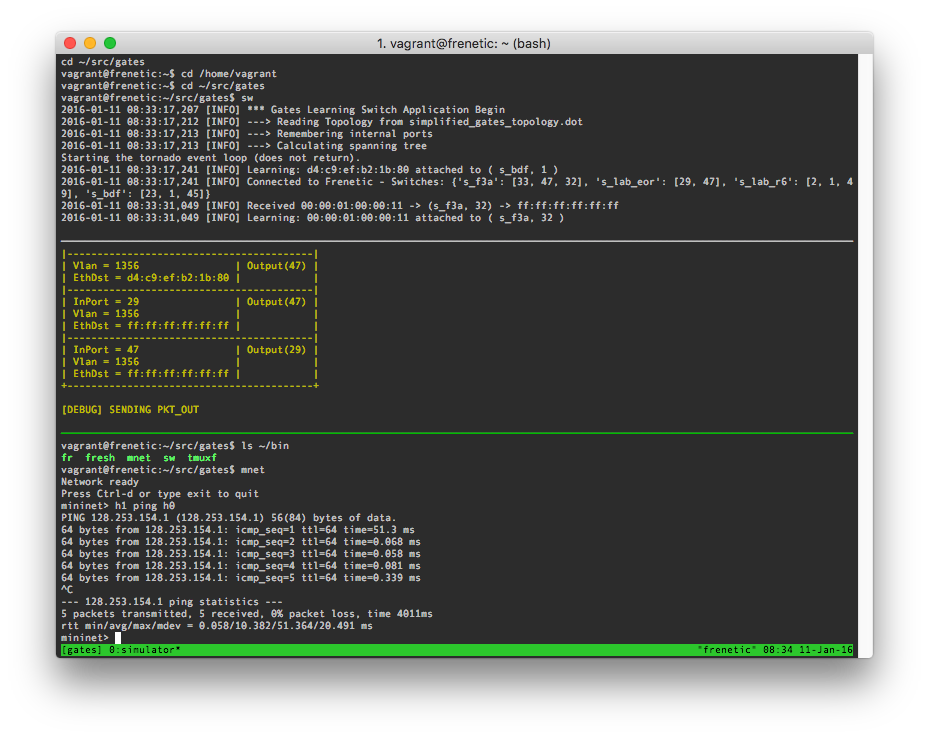
\includegraphics[scale=0.4]{tmux_example}

In Frenetic development, it's helpful to run tmux with at least 3 panes, which you can see in the example above:

\begin{enumerate}
\item One pane runs your network application, e.g. \netkat{python repeater.py}
\item One pane runs Frenetic, e.g. \netkat{frenetic http-server --verbosity debug}
\item One pane runs Mininet
\end{enumerate}

Tmux is very personalizable and configurable.  
But if you haven't used tmux before, here is a good setup to get you started.

\begin{enumerate}
\item Install tmux on Frenetic-vm with \netkat{sudo apt-get install tmux}
\item Create a file in your home directory, ./tmux.conf with the line \netkat{set -g prefix C-a}.  
This maps the tmux prefix key to \Ctrl+\keystroke{A}, which is much easier to reach than the default 
\Ctrl+\keystroke{B}
\item Type \netkat[style=BashInputStyle]{tmux} to start.
\end{enumerate}

\Ctrl+\keystroke{A} is called the \emph{prefix key}, and we'll denote it as \keystroke{Prefix} below. 
Because you will be typing the prefix a lot, it's really helpful to map your \keystroke{Caps Lock} key to \Ctrl, if
you haven't already done so.  
On a Mac, for example, you can go to Apple Menu $\rightarrow$ System Preferences $\rightarrow$ Keyboard 
$\rightarrow$ Keyboard Tab $\rightarrow$ Modifier Keys and select Control for Caps Lock.

Once there, you can use the following key combinations:

\begin{itemize}
\item \keystroke{Prefix} \keystroke{=} splits the pane at the cursor into two panes: one above the cursor and one below.  
You can split existing panes as many times as you want, all the way down to panes with one line (which are probably
not very useful).   
\item \keystroke{Prefix} \UArrow moves the cursor to the pane above.
(If you're on the top pane already, the cursor moves to the bottom-most pane.)
\item \keystroke{Prefix} \DArrow moves the cursor to the pane below.
(If you're on the bottom pane already, the cursor moves to the top-most pane.)
\item \keystroke{Prefix} \keystroke{Z} zooms the current pane, so that it takes up the entire window. 
The other panes continue to run, even though they're not visible.
Pressing \keystroke{Prefix} \keystroke{Z} again unzooms the window.  
\item \keystroke{Prefix} \keystroke{D} detaches from the Tmux session.  
You can start it up again later, even after having logged off the Frenetic VM, by using 
\netkat{tmux attach}.
\end{itemize}

Because tmux operates outside the normal window manager realms, you can no longer scroll up or down
in a pane using scroll bars.  
But tmux has a scrolling mechanism inside itself which scrolls panes independently.  

\begin{itemize}
\item \keystroke{Prefix}, \keystroke{[} enters scroll mode.  
You can see a cursor position status at the top right hand corner of the pane: 67/900 means you're
on line 67 of 900 lines in the pane.   
\item once in scroll mode:
\begin{itemize}
\item \UArrow moves the cursor one line up.
\item \DArrow moves the cursor one line down.
\item \PgUp moves the cursor one page up.
\item \PgDown moves the cursor one page down.
\item\Esc leaves scroll mode and scrolls all the way down to the bottom
\end{itemize}
\end{itemize}

If you end up doing the same keystrokes each time you start up an SDN session, you can automate it
with tmuxinator software.

The book \citet{hogan:tmux} is a great introduction and reference to tmux.  

\section{Open VSwitch Utilities}

\section{TCPDump}
 \label{sdn_development_tools:tcpdump}

\section{Mininet Network Modelling}


\chapter{Network Address Translation}

\section{Why Do We Need NAT?}
 \label{network_address_translation:why_needed}

\section{Design}


\chapter{Spanning Tree Alternatives}

\section{What's Wrong with STP Protocols?}
 \label{spanning_tree:whats_wrong}

\section{Design}

\section{Calculating Shortest Paths}

\section{Core/Edge Separation}



% !TEX root = frenetic_programmers_guide.tex

\chapter{Routing}

\section{Design}
\label{routing:design}

Up until now, we've been dealing with OSI Layer 2 technologies -- those that operate at the
Ethernet packet level.  Now we'll step one layer up the stack to Layer 3: Internet Protocol
or IP.  

From the IP perspective, the Internet is just a bunch of LAN's organized into networks, 
then further divided into subnets.  For our purposes, we'll concentrate on
IP Version 4 or IPv4, which is currently the most popular of the two IP versions (the other being
IP Version 6 or IPv6).  

A particular IPv4 address, for example 10.0.1.3, may be part of a subnet
with other hosts.  We may set up a subnet labelled 10.0.1.0/24, which means the first 24 bits
comprise the subnet number, and the last $32 - 24 = 8$ bits are the host number.  In our example, the
subnet number is 10.0.1 and the host is 3.  Because the host number is 8 bits, this means our example
host lives in a subnet with up to 256 neighbors.  Some neighbors are reserved:

\begin{description}
\item[Host 0] in this case 10.0.1.0, usually has no host assigned to it. 
\item[Host 1] in this case 10.0.1.1, is usually the default gateway of the subnet, which we'll see in 
a minute.
\item[Host $n$ - 1] in this case 10.0.1.255, is the subnet broadcast address.
\end{description}

This leaves you with $n$ - 3 ``real'' neighbor hosts.  You can think of a subnet as a gated community
where the most common action is to talk with your neighbors, but not with those outside your
subnet.  To do the latter, you need an intermediary \ldots in IP, that intermediary is a router.

So suppose we have two subnets, each with two hosts, organized like this:

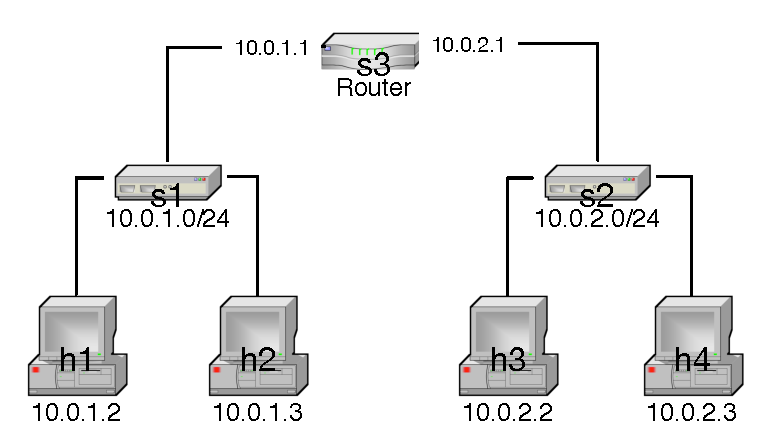
\includegraphics{routing_topo.pdf}

There is no such thing as speaking IP \emph{natively} over a network.  You must speak the wire protocol,
which in most cases is Ethernet.  Because IP applications like your browser and Ping can only speak
in IP addresses, there must be a translation mechanism between IP addresses and Ethernet addresses.
That translation mechanism is Address Resolution Protocol or ARP.  

A typical conversation between two hosts on the same subnet, looks something like this:

\begin{enumerate}
\item Host 10.0.1.2 wants to communicate with 10.0.1.3, but doesn't know its MAC address.
\item It broadcasts over Ethernet an ARP request, "Who has 10.0.1.3" ?
\item If it's up, 10.0.1.3 sends back an ARP reply, "10.0.1.3 is at 11:22:33:44:55:66", which is
presumably its own MAC address.
\item Host 10.0.1.2 then constructs an Ethernet packet with destination 11:22:33:44:55:66 and sends it off.
\end{enumerate}

We haven't had to think about ARP in previous chapters, because the hosts have seamlessly handled it
for us.  Our L2 learning switch handles Ethernet broadcasts and Ethernet unicasts just fine, so every
part of the conversation above was handled by it seamlessly.

Now, throw a router into the mix and the conversation gets slightly more complicated.  Host IP
stacks distinguish between hosts on their own subnet and hosts on other subnets.  If
10.0.1.2 wants to talk to 10.0.2.3, the host won't just send out an ARP request for 10.0.2.3 -- it's
on another network.  Hosts can have routing tables to tell it where to direct inter-network
traffic, but in most cases the routing table contains one entry: the default gateway.  The default
gateway is usually set by DHCP, but it's generally a special IP address on the subnet where the
router lives. In this case the conversation becomes:

\begin{enumerate}
\item Host 10.0.1.2 wants to communicate with 10.0.2.3, but doesn't know it's MAC address.  Since
10.0.2.3 is on different subnet, and there's no routing table entry for a subnet including 10.0.2.3,
it decides to send to a default gateway 10.0.1.1
\item It broadcasts over Ethernet an ARP request, ``Who has 10.0.1.1?''
\item The router sends back an ARP reply, "10.0.1.1 is at 11:00:00:00:00:00", which is
the MAC address of the router port responsible for subnet 10.0.1.0/24.
\item Host 10.0.1.1 then constructs an Ethernet packet with destination 11:00:00:00:00:00 and sends it off.
\end{enumerate}

And now the router can do its thing:

\begin{enumerate}
\item The destination IP is 10.0.2.3, and the router knows it has subnet 10.0.2.0/24
on port 2.  But it doesn't know the MAC address of 10.0.2.3.
\item The router broadcasts an ARP request over port 2 ``Who has 10.0.2.3?''
\item That host responds with an ARP reply ``10.0.2.3 is at ff:ee:dd:cc:bb:aa'', which is its 
own MAC address.
\item Router constructs an Ethernet packet with the router MAC address connected to that
subnet as its source,
and ff:ee:dd:cc:bb:aa as its destination and sends it off.
\end{enumerate}

A couple of things to note are:

\begin{itemize}
\item Only IP traffic gets routed.  
\item Only Ethernet sources and destinations are changed in the packet.  The IP addresses
stay the same no matter where they are in the journey.
\item A router must buffer packets until the ARP replies return.  For subsequent requests, it caches the
IP-to-MAC translation, like a learning switch does with MACs.
\item If the router receives a packet bound for a network not directly connected to it, the router
itself has a default gateway it can send to.  
\end{itemize}

So the router does three basic things: answers ARP requests, sends ARP requests, and routes
a packet to the ``next hop''.  Of course real routers do much more than that: they maintain routing tables,
translate network protocols, drop blatantly malicious traffic, and so on.  But we'll concentrate 
on the three core router functions here.

\section{Modeling The Topology}
\label{routing:topo}

Every OpenFlow enabled device is called a \emph{switch}, but you should not confuse it
with a traditional L2 switch.  An OpenFlow switch can model just about any network device
including firewalls, load balancers, and -- as we'll see in this chapter -- routers.  

In Chapter \ref{chapter:multiswitch_topologies}, we saw two ways of modeling the network topology:
statically with a \netkat{.dot} file and dynamically via Frenetic.  One advantage of a
static topology is you can share it between Mininet and your application.  That 
way you can model more difficult topologies completely, and only change one file
to change the design.  

So here is our DOT file, from \codefilename{routing/topology.dot}:

\inputminted{python}{code/routing/topology.dot}

We've added a few more attributes to accommodate IP.  In particular:

\begin{description}
\item[router] is set to true on the device acting as the router
\item[ip] addresses are assigned to each host 
\item[gateway] addresses is the default gateway to which the host sends packets.  All packets not
bound for hosts in the same subnet go here.   
\end{description}

Here's the GraphViz generated diagram from the above:

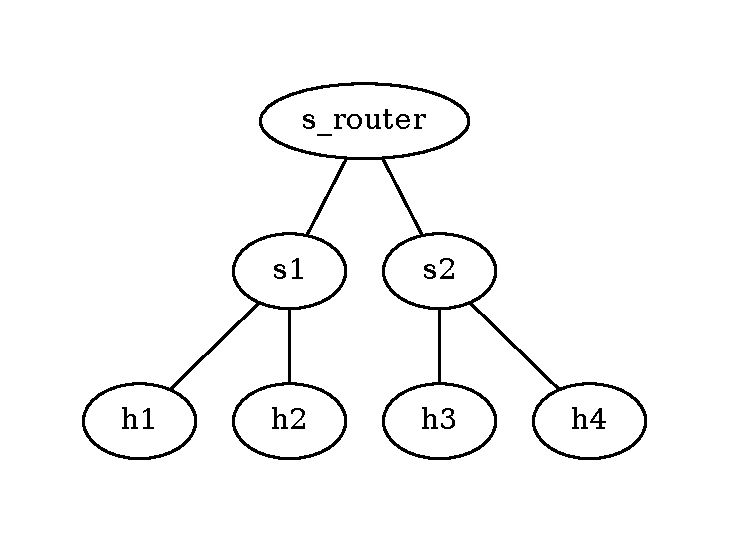
\includegraphics{routing_topology.pdf}

Like we did in previous chapters,  we
can define a custom Mininet toplogy by writing some Python code calling the Mininet
API's.  

The following code is in \codefilename{routing/mn_dot_topology.py}:

\inputminted{python}{code/routing/mn_dot_topology.py}

This program relies on the \python{agraph} API, which we used in 
hapter \ref{chapter:handling_vlans}, and 
the Mininet API, documented at: http://mininet.org/api/annotated.html.  The interesting calls are:

\begin{description}
\item[addSwitch()] which adds a new Mininet switch with a particular DPID.
\item[addHost()] which adds a host
\item[addLink()] which adds virtual ``wire'' between a host and a switch, or two switches.
\end{description}

In this program, we're careful to set the port ids to some defaults.  Although that's not
technically necessary, since L2 learning will establish a table of MAC-to-port mappings,
it makes debugging easier.    

To run this Mininet topology, you simply run this python file as root:

\begin{minted}{console}
frenetic@ubuntu-1404:~/manual/programmers_guide/code/routing$ sudo python mn_dot_topology.py
*** Removing excess controllers/ofprotocols/ofdatapaths/pings/noxes

  ... a lot of cleanup messages 

*** Cleanup complete.
Unable to contact the remote controller at 127.0.0.1:6633
Network ready
Press Ctrl-d or type exit to quit
mininet>
\end{minted} 

Finally, we set up a static routing table.   Subnets directly connected to a router are usually 
configured statically in this manner, while indirectly-connected subnet entries are handled by
a route advertising protocol like OSPF.  

We use simple JSON to define the subnets in \codefilename{routing/routing_table.json}:

\inputminted{json}{code/routing/routing_table.json}

This information isn't needed to \emph{build} the network, but it's crucial for its operation.

\section{A Better Router}

One of the problems with traditional routing is the ARP process.  The router must have gobs of memory 
to buffer packets waiting for ARP replies \ldots and those replies may never arrive!  But here, SDN 
can help us build a faster router.

In Chapter \ref{chapter:multiswitch_topologies} we saw how a global network view helps us build a loop-free
network without the hassle of spanning tree.  We can use this same global network view to build
routing without relying as much on ARP.  

The key is in the L2 learning tables.  If 10.0.1.2 wants to communicate with 10.0.2.3, we probably know
both of their MAC addresses.  10.0.1.2 cannot simply address its packet directly to that MAC because
it's not on the same switch (and Ethernet, by itself, is not routable).  But the router can use 
10.0.2.3's MAC address to perform the second hop.  It can skip the buffering and ARP request step
altogether.

But what if the MAC address of 10.0.2.3 is \emph{not} known?  
This looks like the case in the L2 learning switch when we simply ``punt'' and flood the packet
over all ports.  
Unfortunately the router can't do that with L3 packets.  If you simply stamp an Ethernet broadcast
address in the same packet as the destination IP, the end hosts will see the packet, note that 
the IP and MAC addresses don't match, and drop the packet.
In this case, the router \emph{does} need
to enqueue packets, send the ARP request, monitor the response, and release the packets when 
their destination MAC is known.   

Under these conditions, the L2 switches need very few modifications.  When a host needs to send an 
internetwork packet, it always starts by sending the packet to the default gateway.  From that 
perspective, the default gateway is no different than any other host.  If the sender knows 
its MAC address, it simply sends it.  If it doesn't, it broadcasts an ARP request for it and the
router responds.  

The router needs to implement a rule for each learned MAC in the network.  For each
$mac$ and address $ip$, you first determine the router port $rp$ and the MAC address of that
port $rtrmac$.  That can be calculated since
we know which subnet is connected to each router port.  Then we write the rule:

\begin{minted}{python}
Filter(EthTypeEq(0x800) & IP4DstEq(ip)) >> \
  SetEthSrc(rtrmac) >> SetEthDst(mac) >> SetPort(rp) 
\end{minted}

Two more things: we need to catch all remaining unlearned IP destinations, and 
we need to catch all ARP requests so that we can answer requests for the default gateway:

\begin{minted}{python}
Filter(EthTypeEq(0x800, 0x806) ) >> SendToController("router") 
\end{minted}

Note that we don't need to \emph{answer} all ARP requests, necessarily \ldots and in fact we'll see
ARP requests for intra-network hosts because they are broadcast over the subnet.  We can ignore those
since they'll be answered by the host itself.  The only ones we reply to are those for the default 
gateway.  

\section{Modularization}

When we get done, our network application will perform the job of both the switches and the router.  
Up until now, we have written our applications as one subclass of \python{Frenetic.App}, but here
it makes sense to modularize the application into a switch part and a router part.  We call these
\emph{handlers}, and they implement the same method signatures that Frenetic applications do.  
They are not subclasses of \python{Frenetic.App} -- making them subclasses would give them each 
their own event loops and asynchronous calls, which simply makes things too complicated.   However, 
because the method signatures are identical, the surrounding classes
could be turned into their own freestanding Frenetic applications.

The main application looks like this, from \codefilename{routing/routing1.py}:

\inputminted{python}{code/routing/routing1.py}

Notice how it creates one NIB, and passes these to both switch and router handlers.  This allows
them to share state.  But learning a new MAC on the switch should trigger a policy recalculation on
the router.  Rather than coding this dependency into the router (which then couples it to the switch 
handler), we handle the recalculation here.  

The recalculation uses a trick from the Tornado Python library.  If you simply call the 
\python{update_and_clear_dirty()} function, many successive packets may cause the updates to 
happen in a random order since the requests are handled asynchronously.  This can cause older
calculated rules sets to overwrite newer ones.  By using \python{IOLoop.add_timeout()}, we enqueue
all the recalculations so they occur in order.  

There's not a lot of code in this app -- most of the actual work is delegated to the handlers
\python{SwitchHandler} and \python{RouterHandler}.  Each handler does two main tasks: (a) review
incoming packets and (b) contribute their portion of the network-wide policy based on the NIB.  
Since the switches and router policies are non-overlapping (they have different \netkat{SwitchEq} filters)
simply \netkat{Union}'ing them together gives you the network-wide policy.  
In this app, all the handler workflow is hard-coded, but you can imagine a more dynamic 
main program that would register handlers and dynamically delegate events based on signatures. 
That's overkill for our routing application.

The NIB, in \codefilename{routing/network_information_base.py} looks a lot like the NIB
we use in multiswitch handling.  IP information, though, makes the tables a bit wider, 
so we move to using objects instead of tuples.  These two classes model devices (connected hosts
and gateways) and subnets.    

\inputminted[firstline=5,lastline=31]{python}{code/routing/network_information_base.py} 

The hosts table is now a dictionary of MAC addresses to \python{ConnectedDevice} instances. 

The initialization procedure reads the fixed configuration from the Routing Table and topology
files.  It follows the same general outline as the Mininet custom configurator.

\inputminted[firstline=56,lastline=87]{python}{code/routing/network_information_base.py} 

The learning procedure adds the IP field, which may be passed in as \python{None}
for non-IP packets.  The first packet from a device might very well be non-IP, as in a DHCP 
request (even though DHCP asks for an IP address, the DHCP packet itself is not an IP packet).
That might trigger learning on the L2 switch, which records its port and MAC, but no IP address.  
The router can later call this procedure to fill in the missing IP.  

The NIB now has a \python{dirty} flag
which learning/unlearning a MAC can set or reset.  
The main handler uses this to determine whether to do 
a wholesale recalculation of the switch and router policies.

\inputminted[firstline=186]{python}{code/routing/network_information_base.py} 

The switch handler is virtually identical to the switching application of 
Chapter \ref{chapter:multiswitch_topologies}.  
The main difference is extra handling in the MAC learning procedure -- if the packet is an
IP packet, we extract the extra IP address and learn that as well.  One important except is the 
\emph{internal port}, meaning any ports connected to other switches or routers.  Because the 
routing process changes the Ethernet Source MAC, we can't count on it to match the Source IP address,
which itself never changes.  So though we learn the MAC and port of an internal port, we ignore the
IP address of any packets arriving there.  

This code is from \codefilename{routing/switch_handler.py}:

\inputminted[firstline=33]{python}{code/routing/switch_handler.py}

The interesting processing happens in \codefilename{routing/router_handler.py}. First, we set up 
objects to hold queued packets waiting for an ARP reply:

\inputminted[firstline=8,lastline=12]{python}{code/routing/router_handler.py} 

Policies are constructed from the learned MAC table, similarly to the switches.  The big difference
is we look at the entire network-wide MAC table, and we look only at those entries with IP 
addresses.

\inputminted[firstline=24,lastline=53]{python}{code/routing/router_handler.py} 

Here you can see the learned MAC policies, the catch-all subnet policies, and the ARP policy are 
installed.  ARP replies are constructed from scratch using the Frenetic Packet object described in
Section \ref{introduction:packet_in}:

\inputminted[firstline=94,lastline=110]{python}{code/routing/router_handler.py} 

The Packet In handler deals primarily with ARP requests and replies:

\inputminted[firstline=111,lastline=147]{python}{code/routing/router_handler.py} 

And with IP packets:

\inputminted[firstline=149]{python}{code/routing/router_handler.py} 

The queuing and dequeuing procedures are straightforward.  Note that a huge stream of packets to a 
disconnected IP address could easily overwhelm this implementation, and so caps on the queues should
probably be enforced:

\inputminted[firstline=54,lastline=92]{python}{code/routing/router_handler.py} 

\section{Summary}

Routing is more than just forwarding packets to the next subnet.  It also involves support functions
for subnets that connect to it, like ARP and security.  Our network application successfully supplies
those functions.  And in a way, the net apps' global view of the network does routing better than
a traditional router.   When a host connects to it on one side of the network, the hosts 
on the other side take advantage of that knowledge.

Routing is a powerful paradigm for Layer 3 and Layer 4 communications.  In the next chapter, we
extend the concept into Load Balancing, which routes but also rewrites IP addresses along the 
way.  
\chapter{Modularization}

\section{Sharing Actions in Rules and Packet Outs}
 \label{modularization:sharing_predicates}

\section{Subclassing}

\section{Multiple Network Apps}

\section{Clustering}


% !TEX root = frenetic_programmers_guide.tex

\chapter{Frenetic REST API}

The Frenetic Python language bindings are only one way to write network applications.  The Frenetic
HTTP Controller accepts NetKAT policies, configuration settings through JSON, and pushes network
events like Packet In's through JSON.  So any programming language that can speak HTTP and JSON (pretty
much all of them) can talk to Frenetic.  

\section{REST Verbs}
\label{frenetic_rest_api:urls}

The following verbs are implemented in the HTTP Controller:

\bigskip
\begin{tabularx}{\linewidth}{lXX}
\texttt{POST /$client\_id$/update\_json} & Update the network-wide NetKAT policy, compile the tables, and send the
resulting tables to the switches. \\
\texttt{GET /$client\_id$/event} & Get the latest waiting network events \\
\texttt{GET /current\_switches} & Return a list of connected switches and ports \\
\texttt{POST /pkt\_out} & Send a packet out via OpenFlows Packet Out message \\
\texttt{GET /version} & Return Frenetic version \\
\texttt{GET/config} & Get current Frenetic configuration \\
\texttt{POST /config} & Update current Frenetic configuration \\
\texttt{GET /query/$name$} & Get current statistics bucket contents \\
\texttt{GET /port\_stats/$sw$/$port$} & Get port statistics contents for switch $sw$ and port $port$ \\
\texttt{POST /$client\_id$/update} & Same as \texttt{update\_json} but the policy is in Raw NetKAT format 
\end{tabularx}

Of these verbs, you'll be calling \netkat{update_json} and \netkat{event} the most, so we'll discuss 
these in detail.  The rest are outlined in Section \ref{reference:commands}.

\section{Pushing Policies}

You push policies to Frenetic by using the \texttt{POST /$client\_id$/update\_json} verb.  The 
$client\_id$ is identical to the $client\_id$ instance variable set in our Python language examples.
To make the policy updates smaller, you can split the policy into multiple client id's, then 
call \netkat{update\_json} on just that portion to update the policy.   Frenetic recompiles all the
policies together with an implicit \netkat{Union} -- so there can be no overlapping rules in each 
of the clients.  

The data you push is a JSON representation of the NetKAT policy.  For example, this policy using
the Python bindings:

\begin{minted}{python}
Filter(PortEq(1)) >> SetPort(2) |
Filter(PortEq(2)) >> SetPort(1) 
\end{minted}

Will look like this in JSON:

\begin{minted}{json}
{  "type": "union",
   "pols": [
     { "type": "seq",
       "pols": [
         { "type": "filter", 
           "pred": { 
              "type": "test", 
              "header": "port",
              "value": { "type": "physical", "port": 1 }
           }
         },
         { "type": "mod",
           "header": "port",
           "value": { "type": "physical", "port": 2 }
         }
       ]  
     },
     { "type": "seq",
       "pols": [
         { "type": "filter", 
           "pred": { 
              "type": "test", 
              "header": "port",
              "value": { "type": "physical", "port": 2 } 
           }
         },
         { "type": "mod",
           "header": "port",
           "value": { "type": "physical", "port": 1 }
         }
       ]  
     }
   ]
}
\end{minted}

Figuring out the JSON by hand is pretty laborious.  So you can make the Python REPL and Frenetic 
bindings do the work for you like this:

\begin{minted}{console}
vagrant@frenetic:~$ python
Python 2.7.6 (default, Jun 22 2015, 17:58:13)
[GCC 4.8.2] on linux2
Type "help", "copyright", "credits" or "license" for more information.
>>> import frenetic
>>> from frenetic.syntax import *
>>> pol = Filter(PortEq(1)) >> SetPort(2) | Filter(PortEq(2)) >> SetPort(1)
>>> pol.to_json()
{'pols': [{'pols': [{'pred': {'header': 'location', 'type': 'test', 'value': 
{'type': 'physical', 'port': 1}}, 'type': 'filter'}, {'header': 'location', 
'type': 'mod', 'value': {'type': 'physical', 'port': 2}}], 'type': 'seq'}, 
{'pols': [{'pred': {'header': 'location', 'type': 'test', 'value': {'type': 
'physical', 'port': 2}}, 'type': 'filter'}, {'header': 'location', 'type': 
'mod', 'value': {'type': 'physical', 'port': 1}}], 'type': 'seq'}], 'type': 
'union'}
>>>
\end{minted}

The complete catalog of JSON syntax for NetKAT predicates and policies is in Chapter 
\ref{netkat_reference}

\section{Incoming Events}

Calling the \texttt{GET /$client\_id$/event} verb gets a list of incoming network events.
The call will block until events become available, which is why the Python bindings are 
implemented asynchrononously through callbacks.   The events come back as a 
JSON array, so there could be more than one.

All incoming events are listed in Section \ref{netkat_reference:events}.  The most
prevalent one is \netkat{packet_in}, so your call to \texttt{GET /$client\_id$/event} might
return something like this:

\begin{minted}{json}
[
  { "type": "packet in", 
    "switch id": 1981745, 
    "port id": 1, 
    "payload": {
      "id": 19283745, 
      "buffer": "AB52DF57B12BF87216345" 
    }
  }
  { "type": "packet in", 
    "switch id": 923462, 
    "port id": 2, 
    "payload": {
      "buffer": "AB52DF57B12BF87216345" 
    }
  },
]
\end{minted}

The payload may be either buffered or unbuffered -- the absence of an \netkat{id} attribute 
indicates the packet is unbuffered, in which case the \netkat{buffer} attribute is the entire
contents of the packet.  (See Section \ref{intro:buffering} for an explanation of how buffering
works.)

The contents are encoded in Base 64, and most languages have decoders for this type.  You will
need to write or acquire a packet parser to extract and test data from inside the packet -- RYU's
packet library is good on the Python side. 
% !TEX root = frenetic_programmers_guide.tex

\chapter{Frenetic/NetKAT Reference}
\label{netkat_reference}

\section{NetKAT Predicates}
\label{netkat_reference:predicates}

\subsection{Primitives}

\subsubsection{Drop}

\bigskip
\begin{tabularx}{\linewidth}{lX}
\textsc{Python}   & \texttt{Drop} \\
   & \texttt{false} \\ \\
\textsc{Raw}    & \texttt{false}  \\ \\
\textsc{REST} & \texttt{ \{ "type": "false" \} } 
\end{tabularx}

\python{Drop} matches no packets.  This is a \emph{predicate}, as opposed to the lower-case 
equivalent \python{drop} 
which is a \emph{policy} that drops all packets. 

Note in Python, \python{Id} and \python{Drop} are the only predicates that don't require parantheses.

\subsubsection{EthDst}

\bigskip
\begin{tabularx}{\linewidth}{lXX}
\textsc{Python}   & \texttt{EthDstEq("72:00:08:bc:5f:a0")}    & \texttt{EthDstNotEq("72:00:08:bc:5f:a0")} \\
    & \texttt{EthDstEq("72:00:08:bc:5f:a0", "82:9b:41:a6:16:f8")}  & \texttt{EthDstNotEq("72:00:08:bc:5f:a0", "82:9b:41:a6:16:f8")} \\
    & \texttt{EthDstEq(["72:00:08:bc:5f:a0", "82:9b:41:a6:16:f8"])}  & \texttt{EthDstNotEq(["72:00:08:bc:5f:a0", "82:9b:41:a6:16:f8"])} \\ \\
\textsc{Raw}    & \texttt{ethDst = 125344472129440}     & \\ \\
\textsc{REST} & \multicolumn{2}{l}{\texttt{ \{ "type": "test", "header": "ethdst", "value": 125344472129440 \} }} 
\end{tabularx}

\python{EthDstEq} matches packets with a particular Ethernet MAC destination address, or from a set of addresses -- 
if the 
parameter is a list of addresses, there is an implicit OR between them.    

In Python, a MAC address must be specified in colon-separated 6 byte hexadecimal.  This is the most common format
for MAC address display on network devices (although Cisco tends to list them in dotted notation with 2 byte
boundaries).  They must be passed as strings.  In Raw or REST-based NetKAT, you must send the 48-bit MAC as 
an integer.  

\subsubsection{EthSrc}

\bigskip
\begin{tabularx}{\linewidth}{lXX}
\textsc{Python}   & \texttt{EthSrcEq("72:00:08:bc:5f:a0")}    & \texttt{EthSrcNotEq("72:00:08:bc:5f:a0")} \\
    & \texttt{EthSrcEq("72:00:08:bc:5f:a0", "82:9b:41:a6:16:f8")}  & \texttt{EthSrcNotEq("72:00:08:bc:5f:a0", "82:9b:41:a6:16:f8")} \\
    & \texttt{EthSrcEq(["72:00:08:bc:5f:a0", "82:9b:41:a6:16:f8"])}  & \texttt{EthSrcNotEq(["72:00:08:bc:5f:a0", "82:9b:41:a6:16:f8"])} \\ \\
\textsc{Raw}    & \texttt{ethSrc = 125344472129440}     & \\ \\
\textsc{REST} & \multicolumn{2}{l}{\texttt{ \{ "type": "test", "header": "ethsrc", "value": 125344472129440 \} }} 
\end{tabularx}

\python{EthSrcEq} matches packets with a particular Ethernet MAC source address, or from a set of addresses -- 
if the 
parameter is a list of addresses, there is an implicit OR between them.    

In Python, a MAC address must be specified in colon-separated 6 byte hexadecimal.  This is the most common format
for MAC address display on network devices (although Cisco tends to list them in dotted notation with 2 byte
boundaries).  They must be passed as strings.  In Raw or REST-based NetKAT, you must send the 48-bit MAC as 
an integer.  

\subsubsection{EthType}

\bigskip
\begin{tabularx}{\linewidth}{lXX}
\textsc{Python}   & \texttt{EthTypeEq(0x800)}    & \texttt{EthTypeNotEq(0x800)} \\
    & \texttt{EthTypeEq(0x800, 0x806)}  & \texttt{EthTypeNotEq(0x800, 0x806)} \\
    & \texttt{EthTypeEq([0x800, 0x806])}  & \texttt{EthTypeNotEq([0x800, 0x806])} \\ \\
\textsc{Raw}    & \texttt{ethTyp = 2048}     & \\ \\
\textsc{REST} & \multicolumn{2}{l}{\texttt{ \{ "type": "test", "header": "ethtype", "value": 2048 \} }} 
\end{tabularx}

\python{EthType} matches packets with a particular Ethernet frame type, or from a set of frame types -- if the
parameter is a list of types, there is an implicit OR between them.  The frame type is a 32 bit 
integer as defined by IEEE, and the common ones are listed at 
http://www.iana.org/assignments/ieee-802-numbers/ieee-802-numbers.xhtml

Python can accept any valid 32 bit integer representation for the frame type -- it's common to pass them
as hexadecimal values because they're easy to remember.  You can also use constants defined in 
\python{ryu.packet.ether_types}.  Raw and REST-based NetKAT requires them to be specified in
decimal.

Certain OpenFlow match rules have \emph{dependencies} on the Ethernet type.  
In other words, it requires certain Ethernet type matches to be specified when other fields are matched.  For 
example, if the IPv4 source address is matched, then an Ethernet Type match must also be specified as 
IP, e.g. ethernet type 0x800.  This is not required in NetKAT - the Frenetic compiler will 
automatically compile the correct dependencies for you. 

With VLAN tagged packets, OpenFlow matches the
type of the \emph{enclosed packet}.  So for example, an IP packet wrapped with a VLAN tag will match 
\python{EthType(0x800)} even though the actual Ethernet type of the entire packet is 0x8100 (the 
IEEE 802.1q Ethernet type for VLAN packets).  

\subsubsection{Id}

\bigskip
\begin{tabularx}{\linewidth}{lX}
\textsc{Python}   & \texttt{Id} \\
   & \texttt{true} \\ \\
\textsc{Raw}    & \texttt{true}  \\ \\
\textsc{REST} & \texttt{ \{ "type": "true" \} } 
\end{tabularx}

\python{Id} matches all packets.  This is a \emph{predicate}, as opposed to the lower-case 
equivalent \python{id} 
which is a \emph{policy} that accepts all packets. 

Note in Python, \python{Id} and \python{Drop} are the only predicates that don't require parantheses.

\subsubsection{IPDst}

\bigskip
\begin{tabularx}{\linewidth}{lXX}
\textsc{Python}   & \texttt{IPDstEq("192.168.57.100")}    & \texttt{IPDstNotEq("192.168.57.100")} \\
    & \texttt{IPDstEq("192.168.57.0", 24)}  & \texttt{IPDstNotEq("192.168.57.0", 24)} \\ \\
\textsc{Raw}    & \texttt{ip4Dst = 192.168.57.100}     & \texttt{ip4Dst = 192.168.57.0/24} \\ \\
\textsc{REST} & \multicolumn{2}{l}{\texttt{ \{ "type": "test", "header": "ip4dst",}} \\
   & \multicolumn{2}{l}{\texttt{  "value": \{"addr": "192.168.57.100", "mask": 32 \}} \}} \\
   & \multicolumn{2}{l}{\texttt{ \{ "type": "test", "header": "ip4dst",}} \\
   & \multicolumn{2}{l}{\texttt{  "value": \{"addr": "192.168.57.0", "mask": 24 \}} \}} \\
\end{tabularx}

\python{IPDst} matches packets with a particular IP destination address, or destination network.  It only matches
IP v4 packets, as per Openflow 1.0.  

\python{IPDstEq} cannot accept a list of values as other predicates can.  
Instead, you can specify a subnet -- a range
of IP addresses using a bit mask value.  This is identical to using CIDR format, so that 
\python{IPDstEq("192.168.57.0", 24)} matches IP addresses in subnet \python{192.168.57.0/24} -- e.g. 
IP addresses \python{192.168.57.1} to \python{192.168.57.255}.  Leaving out the subnet mask in Python 
or Raw NetKAT is equivalent to specifiying a mask of 32 - meaning all 32 bits of the IP address are used
in the match.  (The 32 must be explicitly specified in REST-based NetKAT).

\subsubsection{IPProto}

\bigskip
\begin{tabularx}{\linewidth}{lXX}
\textsc{Python}   & \texttt{IPProtoEq(6)}    & \texttt{IPProtoNotEq(6)} \\
    & \texttt{IPProtoEq(6,17)}  & \texttt{IPProtoNotEq(6,17)} \\
    & \texttt{IPProtoEq([6,17])}  & \texttt{IPProtoNotEq([6,17])} \\ \\
\textsc{Raw}    & \texttt{ipProto = 6}     & \\ \\
\textsc{REST} & \multicolumn{2}{l}{\texttt{ \{ "type": "test", "header": "ipproto", "value": 6 \} }} 
\end{tabularx}

\python{IPProtoEq} matches packets with a certain IP Protocol, or set of protocols -- if a list is specified, 
there is an implicit OR between them.  It only matches IP v4 packets, as per OpenFlow 1.0 specs.  

The IP Protocol is a number from 1-255.  A complete list of common protocols are listed in 
https://en.wikipedia.org/wiki/List\_of\_IP\_protocol\_numbers.  In Python, you can also match against the
constants in \python{ryu.packet.in_proto}.

\subsubsection{IPSrc}

\bigskip
\begin{tabularx}{\linewidth}{lXX}
\textsc{Python}   & \texttt{IPSrcEq("192.168.57.100")}    & \texttt{IPSrcNotEq("192.168.57.100")} \\
    & \texttt{IPSrcEq("192.168.57.0", 24)}  & \texttt{IPSrcNotEq("192.168.57.0", 24)} \\ \\
\textsc{Raw}    & \texttt{ip4Src = 192.168.57.100}     & \texttt{ip4Src = 192.168.57.0/24} \\ \\
\textsc{REST} & \multicolumn{2}{l}{\texttt{ \{ "type": "test", "header": "ip4src",}} \\
   & \multicolumn{2}{l}{\texttt{  "value": \{"addr": "192.168.57.100", "mask": 32 \}} \}} \\
   & \multicolumn{2}{l}{\texttt{ \{ "type": "test", "header": "ip4src",}} \\
   & \multicolumn{2}{l}{\texttt{  "value": \{"addr": "192.168.57.0", "mask": 24 \}} \}} \\
\end{tabularx}

\python{IPSrc} matches packets with a particular IP source address, or source network.  It only matches
IP v4 packets, as per Openflow 1.0.  

\python{IPSrcEq} cannot accept a list of values as other predicates can.  
Instead, you can specify a subnet -- a range
of IP addresses using a bit mask value.  This is identical to using CIDR format, so that 
\python{IPSrcEq("192.168.57.0", 24)} matches IP addresses in subnet \python{192.168.57.0/24} -- e.g. 
IP addresses \python{192.168.57.1} to \python{192.168.57.255}.  Leaving out the subnet mask in Python 
or Raw NetKAT is equivalent to specifiying a mask of 32 - meaning all 32 bits of the IP address are used
in the match.  (The 32 must be explicitly specified in REST-based NetKAT).


\subsubsection{Port}

\bigskip
\begin{tabularx}{\linewidth}{lXX}
\textsc{Python} 	& \texttt{PortEq(1)} 		& \texttt{PortNotEq(1)} \\
	 	& \texttt{PortEq(1,2,3)} 	& \texttt{PortNotEq(1,2,3)} \\
	 	& \texttt{PortEq([1,2,3])} 	& \texttt{PortNotEq([1,2,3])} \\ \\
\textsc{Raw}		& \texttt{port = 1} 		& \\ \\
\textsc{REST}	& \multicolumn{2}{l}{\texttt{ \{ "type": "test", "header": "location", }}\\
 & \multicolumn{2}{l}{\texttt{ "value": \{ "type": "physical", "port": 1 \} \} }} 
\end{tabularx}

\python{PortEq} matches packets that arrive on a particular port, or on a particular set of ports -- if the 
parameter is a list of ports, there is an implicit OR between them.  

A port number must be an integer from
1 \ldots 65520, the upper limit of physical port numbers according to the OpenFlow 1.0 spec.  It can also be 
a string convertible to an integer in this range.  The port number is not checked against any known list
of port numbers on the switch, so you can insert rules for non-operational ports (they obviously won't
match any packets until the port becomes operational).  

\python{PortEq} predicates are usually combined with \python{SwitchEq} predicates because packet processing
is switch-and-port-specific.  However, it may be used alone if, for example, a packet on port 47 is processed exactly
the same on every switch (for example, port 47 is the trunk port between switches).  

\subsubsection{Switch}

\bigskip
\begin{tabularx}{\linewidth}{lXX}
\textsc{Python} 	& \texttt{SwitchEq(1981745)} 		& \texttt{SwitchNotEq(1981745)} \\
	 	& \texttt{SwitchEq(1981745, 887345)} 	& \texttt{SwitchNotEq(1981745, 887345)} \\
	 	& \texttt{SwitchEq([1981745, 887345])} 	& \texttt{SwitchNotEq([1981745, 887345])} \\ \\
\textsc{Raw}		& \texttt{switch = 1981745} 		& \\ \\
\textsc{REST}	& \multicolumn{2}{l}{\texttt{ \{ "type": "test", "header": "switch", "value": 1981745 \} }} 
\end{tabularx}

\python{SwitchEq} matches packets that arrive on a particular switch or set of switches.  
Switches are identified by 
a 64-bit number called a \emph{datapath ID} or \emph{DPID}.  On OpenVSwitch, the default OpenFlow
switch provided by Mininet, DPID's are generally small integers corresponding to the switch name --
e.g. \python{s1} in Mininet has the DPID 1.  Physical switches generally append the OpenFlow instance
number with the overall MAC id of the switch so it's globally unique.  But this varies from switch
to switch. 

\python{SwitchEq} predicates are usually combined with \python{PortEq} predicates because packet processing
is switch-and-port-specific.  

\subsubsection{TCPDstPort}

\bigskip
\begin{tabularx}{\linewidth}{lXX}
\textsc{Python}   & \texttt{TCPDstPortEq(80)}    & \texttt{TCPDstPortNotEq(80)} \\
    & \texttt{TCPDstPortEq(80,443)}  & \texttt{TCPDstPortNotEq(80,443)} \\
    & \texttt{TCPDstPortEq([80,443])}  & \texttt{TCPDstPortNotEq([80,443])} \\ \\
\textsc{Raw}    & \texttt{tcpDstPort = 80}     & \\ \\
\textsc{REST} & \multicolumn{2}{l}{\texttt{ \{ "type": "test", "header": "tcpdstport", "value": 80 \} }} 
\end{tabularx}

\python{TCPDstPortEq} matches packets with a certain TCP or UDP destination port, or set of ports -- if the 
parameter is a list of ports, there is an implicit OR between them.  Note this only matches TCP or UDP packets,
which must be IP packets.  A complete list of common destination ports are listed in 
https://en.wikipedia.org/wiki/List\_of\_TCP\_and\_UDP\_port\_numbers

\subsubsection{TCPSrcPort}

\bigskip
\begin{tabularx}{\linewidth}{lXX}
\textsc{Python}   & \texttt{TCPSrcPortEq(5000)}    & \texttt{TCPSrcPortNotEq(5000)} \\
    & \texttt{TCPSrcPortEq(5000,5001)}  & \texttt{TCPSrcPortNotEq(5000,5001)} \\
    & \texttt{TCPSrcPortEq([5000,5001])}  & \texttt{TCPSrcPortNotEq([5000,5001])} \\ \\
\textsc{Raw}    & \texttt{tcpSrcPort = 5000}     & \\ \\
\textsc{REST} & \multicolumn{2}{l}{\texttt{ \{ "type": "test", "header": "tcpsrcport", "value": 5000 \} }} 
\end{tabularx}

\python{TCPSrcPortEq} matches packets with a certain TCP or UDP source port, or set of ports -- if the 
parameter is a list of ports, there is an implicit OR between them.  Note this only matches TCP or UDP packets,
which must be IP packets.  

\python{TCPSrcPort} matches are rarely used in OpenFlow since TCP and UDP source ports are essentially random
numbers assigned by the client.  They can be used for ``per-flow'' rules where a rule lasts for the 
duration of a conversation between a client and a server.  

\subsubsection{Vlan}

\bigskip
\begin{tabularx}{\linewidth}{lXX}
\textsc{Python}   & \texttt{VlanEq(1001)}    & \texttt{VlanNotEq(1001)} \\
    & \texttt{VlanEq(1001,1002)}  & \texttt{VlanNotEq(1001,1002)} \\
    & \texttt{VlanEq([1001,1002])}  & \texttt{VlanNotEq([1001,1002])} \\ \\
\textsc{Raw}    & \texttt{vlanId = 1001}     & \\ \\
\textsc{REST} & \multicolumn{2}{l}{\texttt{ \{ "type": "test", "header": "vlan", "value": 1001 \} }} 
\end{tabularx}

\python{VlanEq} matches packets that arrive with a particular VLAN tag, or on a particular set of VLAN tags -- 
if the 
parameter is a list of vlans, there is an implicit OR between them.  

The VLAN id, as defined by IEE 802.1q is a 12 bit value from 1 \ldots 4095.  VLAN matches are only applicable
to packets with an actual VLAN tag, so the Ethernet Type is 0x8100.  However, in such cases, 
OpenFlow exposes the Ethernet 
Type of the \emph{enclosed packet}.  So for example, an IP packet wrapped with a VLAN tag will match 
\python{EthType(0x800)}.  

In most physical switches, access ports are tagged with a particular VLAN.  So though the packet coming
from the host is untagged, the tagging occurs at the switch before the OpenFlow engine is invoked.  
That way you can assign access ports to VLANs, and any packets coming in on that port will match the
appropriate \python{VlanEq}.  This is one of the few cases where packet headers are manipulated outside the
OpenFlow engine.  

\subsubsection{VlanPcp}

\bigskip
\begin{tabularx}{\linewidth}{lXX}
\textsc{Python}   & \texttt{VlanPcpEq(1)}    & \texttt{VlanPcpNotEq(1)} \\
    & \texttt{VlanPcpEq(1,2)}  & \texttt{VlanPcpNotEq(1,2)} \\
    & \texttt{VlanPcpEq([1,2])}  & \texttt{VlanPcpNotEq([1,2])} \\ \\
\textsc{Raw}    & \texttt{vlanPcp = 1}     & \\ \\
\textsc{REST} & \multicolumn{2}{l}{\texttt{ \{ "type": "test", "header": "vlanpcp", value: 1 \} }} 
\end{tabularx}

\python{VlanPcpEq} matches packets that arrive with a particular VLAN Priority Code Point (PCP), 
or on a particular set of VLAN PCP's -- 
if the 
parameter is a list of PCP's, there is an implicit OR between them.  Only VLAN tagged packets
will match this predicate.

The PCP as defined by IEEE 802.1q must be an integer from 0-7.  0 is the default, generally meaning
best effort delivery.  

\subsection{Combinations}

\subsubsection{And}

\bigskip
\begin{tabularx}{\linewidth}{lX}
\textsc{Python}   & \texttt{$pred_1$ \& $pred_2$} \\
    & \texttt{And([$pred_1$, $pred_2$, \ldots, $pred_n$])} \\ \\
\textsc{Raw}    & \texttt{$pred_1$ and $pred_2$}  \\ \\
\textsc{REST} & \texttt{ \{ "type": "and", "preds": [ $pred_1$, $pred_2$, \ldots $pred_n$ ] \} } 
\end{tabularx}

\python{And} is the Boolean conjunction of predicates. 

\subsubsection{Not}

\bigskip
\begin{tabularx}{\linewidth}{lX}
\textsc{Python}   & \texttt{\textasciitilde $pred_1$} \\
    & \texttt{Not($pred_1$)} \\ \\
\textsc{Raw}    & \texttt{not $pred_1$}  \\ \\
\textsc{REST} & \texttt{ \{ "type": "neg", "pred": $pred_1$ \} } 
\end{tabularx}

\python{Not} is the Boolean negation of a single predicate.

\subsubsection{Or}

\bigskip
\begin{tabularx}{\linewidth}{lX}
\textsc{Python}   & \texttt{$pred_1$ $\vert$ $pred_2$} \\
    & \texttt{Or([$pred_1$, $pred_2$, \ldots, $pred_n$])} \\ \\
\textsc{Raw}    & \texttt{$pred_1$ or $pred_2$}  \\ \\
\textsc{REST} & \texttt{ \{ "type": "or", "preds": [ $pred_1$, $pred_2$, \ldots $pred_n$ ] \} } \end{tabularx}

\python{Or} is the Boolean disjunction of predicates.  In Python, if all of your disjunction terms involve
the same field, you can use the list form of the simple predicate as a shortcut (except for 
\python{IpSrcEq} and \python{IpDstEq}). 

Note that in Python \python{Or} shares a symbol with \python{Union}, but the parser keeps the meaning straight.

\section{Policies}

\subsection{Primitives}

\subsubsection{drop}

\bigskip
\begin{tabularx}{\linewidth}{lX}
\textsc{Python}   & \texttt{drop} \\ \\
\textsc{Raw}   & \texttt{drop} \\ \\
\textsc{REST} & \texttt{ \{ "type": "filter", "pred": \{ "type": false \} \} } 
\end{tabularx}

\python{drop} is a \emph{policy} that drops all packets.  It is equivalent to \python{Filter(false)}.

Note that in Python, \python{id} and \python{drop} are the only policies that begin with a lower case
letter, and do not require parantheses.  

\subsubsection{Filter}

\bigskip
\begin{tabularx}{\linewidth}{lX}
\textsc{Python}   & \texttt{Filter($pred$)} \\ \\
\textsc{Raw}   & \texttt{filter $pred$} \\ \\
\textsc{REST} & \texttt{ \{ "type": "filter", "pred": $pred$ \} } 
\end{tabularx}

\python{Filter} accepts all packets that match the predicate $pred$ and rejects everything else.
It is described in detail in Section \ref{section:combining}.

\subsubsection{id}

\bigskip
\begin{tabularx}{\linewidth}{lX}
\textsc{Python}   & \texttt{id} \\ \\
\textsc{Raw}   & \texttt{id} \\ \\
\textsc{REST} & \texttt{ \{ "type": "filter", "pred": \{ "type": true \} \} } 
\end{tabularx}

\python{drop} is a \emph{policy} that drops all packets.  It is equivalent to \python{Filter(true)}.

Note that in Python, \python{id} and \python{drop} are the only policies that begin with a lower case
letter, and do not require parantheses.  

\subsubsection{SendToController}

\bigskip
\begin{tabularx}{\linewidth}{lX}
\textsc{Python}   & \texttt{SendToController("http")} \\ \\
\textsc{Raw}    & \texttt{port := pipe("http")}     \\ \\
\textsc{REST} & \texttt{ \{ "type": "mod", "header": "location", } \\
 & \texttt{ "value": \{ "type": "pipe", "name": "http" \} \} } 
\end{tabularx}

\python{SendToController} sends the packet to the controller.   

The pipe name is an arbitrary string.  You can use it to distinguish \ldots

\begin{quotation}
\emph{Note: I'm not sure how you distinguish packets using pipes since they're not part of the 
packet and you can't do matches on them.}
\end{quotation}

\subsubsection{SendToQuery}

\bigskip
\begin{tabularx}{\linewidth}{lX}
\textsc{Python}   & \texttt{SendToQuery("internet")} \\ \\
\textsc{Raw}    & \texttt{port := query("internet")}     \\ \\
\textsc{REST} & \texttt{ \{ "type": "mod", "header": "location", } \\
 & \texttt{ "value": \{ "type": "query", "name": "internet" \} \} } 
\end{tabularx}

\python{SendToQuery} counts packets and bytes that meet certain match criteria.  This is described in
Section \ref{statistics:queries}.   


\subsubsection{SetEthDst}

\bigskip
\begin{tabularx}{\linewidth}{lX}
\textsc{Python}   & \texttt{SetEthDst("72:00:08:bc:5f:a0")} \\ \\
\textsc{Raw}    & \texttt{ethDst := 125344472129440}     \\ \\
\textsc{REST} & \texttt{ \{ "type": "mod", "header": "ethdst", "value": 125344472129440 \} }
\end{tabularx}

\python{SetEthDst} sets the Ethernet MAC destination address for a packet.    

In Python, a MAC address must be specified in colon-separated 6 byte hexadecimal.  This is the most common format
for MAC address display on network devices (although Cisco tends to list them in dotted notation with 2 byte
boundaries).  They must be passed as strings.  In Raw or REST-based NetKAT, you must send the 48-bit MAC as 
an integer.  

\subsubsection{SetEthSrc}

\bigskip
\begin{tabularx}{\linewidth}{lX}
\textsc{Python}   & \texttt{SetEthSrc("72:00:08:bc:5f:a0")} \\ \\
\textsc{Raw}    & \texttt{ethSrc := 125344472129440}     \\ \\
\textsc{REST} & \texttt{ \{ "type": "mod", "header": "ethsrc", "value": 125344472129440 \} }
\end{tabularx}

\python{SetEthDst} sets the Ethernet MAC source address for a packet.    

In Python, a MAC address must be specified in colon-separated 6 byte hexadecimal.  This is the most common format
for MAC address display on network devices (although Cisco tends to list them in dotted notation with 2 byte
boundaries).  They must be passed as strings.  In Raw or REST-based NetKAT, you must send the 48-bit MAC as 
an integer.  

\subsubsection{SetEthType}

\bigskip
\begin{tabularx}{\linewidth}{lX}
\textsc{Python}   & \texttt{SetEthType(0x800)} \\ \\
\textsc{Raw}    & \texttt{ethTyp := 2048}     \\ \\
\textsc{REST} & \texttt{ \{ "type": "mod", "header": "ethtype", "value": 2048 \} }
\end{tabularx}

\python{SetEthType} sets the Ethernet type for a packet.    

Note that for VLAN-tagged packets, you set the Ethernet type for the \emph{inner} packet, not 0x8100
for VLAN.  To tag it with a VLAN, you simply use the policy \netkat{SetVlan}, and that assigns the
correct Ethernet type to the outer packet.  

\subsubsection{SetIPDst}

\bigskip
\begin{tabularx}{\linewidth}{lX}
\textsc{Python}   & \texttt{SetIPDst("192.168.57.100")} \\ \\
\textsc{Raw}    & \texttt{ip4Dst := 192.168.57.100}     \\ \\
\textsc{REST} & \texttt{ \{ "type": "mod", "header": "ip4dst", } \\
  & \texttt{"value": \{"addr": "192.168.57.100" \} \} }
\end{tabularx}

\python{SetIPDst} sets the IP v4 destination address.  Note that unlike the \netkat{IPDstEq} predicate,
there is no option for masking.  You must set a fixed IP address with all bits present.    

The proper Ethernet type for IP packets must already be set in the incoming packet, or through the 
\netkat{SetEthType} policy.  Otherwise, the packet will likely be dropped by a host or router before it 
reaches its destination.

\subsubsection{SetIPProto}

\bigskip
\begin{tabularx}{\linewidth}{lX}
\textsc{Python}   & \texttt{SetIPProto(6)} \\ \\
\textsc{Raw}    & \texttt{ipProto := 6}     \\ \\
\textsc{REST} & \texttt{ \{ "type": "mod", "header": "ipProto", "value": 6 \} }
\end{tabularx}

\python{SetIPProto} sets the IP v4 protocol type.      

The proper Ethernet type for IP packets must already be set in the incoming packet, or through the 
\netkat{SetEthType} policy.  Otherwise, the packet will likely be dropped by a host or router before it 
reaches its destination.

\subsubsection{SetIPSrc}

\bigskip
\begin{tabularx}{\linewidth}{lX}
\textsc{Python}   & \texttt{SetIPSrc("192.168.57.100")} \\ \\
\textsc{Raw}    & \texttt{ip4Src := 192.168.57.100}     \\ \\
\textsc{REST} & \texttt{ \{ "type": "mod", "header": "ip4src", } \\
  & \texttt{"value": \{"addr": "192.168.57.100" \} \} }
\end{tabularx}

\python{SetIPSrc} sets the IP v4 destination address.  Note that unlike the \netkat{IPSrcEq} predicate,
there is no option for masking.  You must set a fixed IP address with all bits present.    

The proper Ethernet type for IP packets must already be set in the incoming packet, or through the 
\netkat{SetEthType} policy.  Otherwise, the packet will likely be dropped by a host or router before it 
reaches its destination.

\subsubsection{SetPort}

\bigskip
\begin{tabularx}{\linewidth}{lX}
\textsc{Python}   & \texttt{SetPort(1)} \\ \\
\textsc{Raw}    & \texttt{port := 1}     \\ \\
\textsc{REST} & \texttt{ \{ "type": "mod", "header": "location", } \\
 & \texttt{ "value": \{ "type": "physical", "port": 1 \} \} } 
\end{tabularx}

\python{SetPort} sets the port destination for this packet.      

A port number must be an integer from
1 \ldots 65520, the upper limit of physical port numbers according to the OpenFlow 1.0 spec.  It can also be 
a string convertible to an integer in this range.  The port number is not checked against any known list
of port numbers on the switch, but any attempt to send a packet over a non-existent or non-operational
port will fail.  

\subsubsection{SetTCPDstPort}

\bigskip
\begin{tabularx}{\linewidth}{lX}
\textsc{Python}   & \texttt{SetTCPDstPort(80)} \\ \\
\textsc{Raw}    & \texttt{tcpDstPort := 80}     \\ \\
\textsc{REST} & \texttt{ \{ "type": "mod", "header": "tcpdstport", "value": 80 \} }
\end{tabularx}

\python{SetTCPDstPort} sets the TCP or UDP destination port.      

The proper Ethernet type for IP packets must already be set in the incoming packet, or through the 
\netkat{SetEthType} policy.  
Also, the proper IP Protocol (TCP or UDP) must already be set in incoming packet, or through the 
\netkat{SetIPProto} policy.  
Otherwise, the packet will likely be dropped by a host or router before it 
reaches its destination.

\subsubsection{SetTCPSrcPort}

\bigskip
\begin{tabularx}{\linewidth}{lX}
\textsc{Python}   & \texttt{SetTCPSrcPort(5000)} \\ \\
\textsc{Raw}    & \texttt{tcpSrcPort := 5000}     \\ \\
\textsc{REST} & \texttt{ \{ "type": "mod", "header": "tcpsrcport", "value": 5000 \} }
\end{tabularx}

\python{SetTCPDstPort} sets the TCP or UDP source port.      

The proper Ethernet type for IP packets must already be set in the incoming packet, or through the 
\netkat{SetEthType} policy.  
Also, the proper IP Protocol (TCP or UDP) must already be set in incoming packet, or through the 
\netkat{SetIPProto} policy.  
Otherwise, the packet will likely be dropped by a host or router before it 
reaches its destination.

\subsubsection{SetVlan}

\bigskip
\begin{tabularx}{\linewidth}{lX}
\textsc{Python}   & \texttt{SetVlan(1001)} \\ \\
\textsc{Raw}    & \texttt{vlanId := 1001}     \\ \\
\textsc{REST} & \texttt{ \{ "type": "mod", "header": "vlan", "value": 1001 \} }
\end{tabularx}

\python{SetVlan} sets the VLAN tag for the packet.  If there is no VLAN tag, it automatically sets 
the \python{EthType} to 0x8100, and pushes the current \python{EthType} into the inner packet.  If there
is already a VLAN tag, it merely overwrites the VLAN id.

\subsubsection{SetVlanPcp}

\bigskip
\begin{tabularx}{\linewidth}{lX}
\textsc{Python}   & \texttt{SetVlanPcp(1)} \\ \\
\textsc{Raw}    & \texttt{vlanPcp := 1}     \\ \\
\textsc{REST} & \texttt{ \{ "type": "mod", "header": "vlanpcp", "value": 1 \} }
\end{tabularx}

\python{SetVlanPcp} sets the VLAN priority for the packet.  If there is no VLAN tag, it automatically sets 
the \python{EthType} to 0x8100, pushes the current \python{EthType} into the inner packet and sets the
VLAN id to 0.  If there
is already a VLAN tag, it merely overwrites the existing VLAN PCP.

\subsection{Combinations}

\subsubsection{IfThenElse}

\bigskip
\begin{tabularx}{\linewidth}{lX}
\textsc{Python}   & \texttt{IfThenElse($pred$, $truepol$ $falsepol$)} \\
\textsc{Raw}    & \texttt{if $pred$ then $truepol$ else $falsepol$}  \\ \\
\end{tabularx}

\python{IfThenElse} tests a predicate and executes $truepol$ if the predicate is true or $falsepol$ if it
is not.  This is explained further in Section \ref{section:combining}.


\subsubsection{Seq}

\bigskip
\begin{tabularx}{\linewidth}{lX}
\textsc{Python}   & \texttt{$pol_1$ >> $pol_2$} \\
    & \texttt{Seq([$pol_1$, $pol_2$, \ldots, $pol_n$])} \\ \\
\textsc{Raw}    & \texttt{$pol_1$ ;  $pol_2$}  \\ \\
\textsc{REST} & \texttt{ \{ "type": "seq", "pols": [ $pol_1$, $pol_2$, \ldots $pol_n$ ] \} } 
\end{tabularx}

\python{Seq} is the sequential composition of policies.  The packet is pushed through each of the
policies one after the other in the order listed.  This is explained further in Section \ref{section:combining}.

\subsubsection{Union}

\bigskip
\begin{tabularx}{\linewidth}{lX}
\textsc{Python}   & \texttt{$pol_1$ $\vert$ $pol_2$} \\
    & \texttt{Union([$pol_1$, $pol_2$, \ldots, $pol_n$])} \\ \\
\textsc{Raw}    & \texttt{$pol_1$ $\vert$  $pol_2$}  \\ \\
\textsc{REST} & \texttt{ \{ "type": "union", "pols": [ $pol_1$, $pol_2$, \ldots $pol_n$ ] \} } 
\end{tabularx}

\python{Union} is the parallel composition of policies.  $n$ copies of the packet are sent through
each of the listed policies in parallel.  This is explained further in Section \ref{section:combining}.

\section{Events}
\label{netkat_reference:events}

In Python, each Frenetic event has a hook listed below.  If the application defines a handler with the same
signature, that handler is called on the event.  If the user doesn't define a handler, a default handler is
invoked which simply logs the event.  

In REST, calling the URL \netkat{/events/$client\_id$} will
return the JSON data below if the event has been fired. 

\subsection{connected}

\bigskip
\begin{tabularx}{\linewidth}{lX}
\textsc{Python}   & \texttt{connected()} \\
\end{tabularx}

There is no \netkat{connected} event in REST.  To simulate it, you simply call GET on the URL \netkat{/version}.  If 
a response comes back (there is no data), then you are connected to Frenetic.

\subsection{packet\_in}

\bigskip
\begin{tabularx}{\linewidth}{lX}
\textsc{Python}   & \texttt{packet\_in($switch\_id$, $port\_id$, $payload$)} \\ \\
\textsc{REST} & \texttt{ \{ "type": "packet\_in", "switch\_id": 1981745, } \\
  & \texttt{"port\_id": 1, "payload": \{ } \\
  & \texttt{"id": 19283745, "buffer": "AB52DF57B12BF87216345" \}\} }
\end{tabularx}

\python{packet_in} is described in detail in Section \ref{introduction:packet_in}.  

In the Python version, $switch\_id$ is a 64-bit DPID per OpenFlow specs,  and $port\_id$ is a 32-bit 
integer.  $payload$ is a Python object of either class \python{Buffered} or \python{NotBuffered}.  
Buffered objects have attributes \python{buffer_id} and\python{buffer} with the decoded data. 
NotBuffered objects only have a \python{data} attribute with the decoded data.    

In the REST version,
the presence of the \python{id} attribute means the packet is Buffered.  The \python{buffer} attribute
is the packet contents encoded in Base64.  

\subsection{port\_down}

\bigskip
\begin{tabularx}{\linewidth}{lX}
\textsc{Python}   & \texttt{port\_down($switch\_id$, $port\_id$)} \\ \\
\textsc{REST} & \texttt{ \{ "type": "port\_down", "switch\_id": 1981745, "port\_id": 1 \} } 
\end{tabularx}

The \python{port_down} event is fired when the port is disconnected, deactivated, reconfigured, or
removed from the OpenFlow engine.  
 
\subsection{port\_up}

\bigskip
\begin{tabularx}{\linewidth}{lX}
\textsc{Python}   & \texttt{port\_up($switch\_id$, $port\_id$)} \\ \\
\textsc{REST} & \texttt{ \{ "type": "port\_up", "switch\_id": 1981745, "port\_id": 1 \} } 
\end{tabularx}

The \python{port_up} event is fired when the port is connected, activated, reconfigured, or
assigned to the OpenFlow engine and is ready to use.  

\subsection{switch\_down}

\bigskip
\begin{tabularx}{\linewidth}{lX}
\textsc{Python}   & \texttt{switch\_down($switch\_id$)} \\ \\
\textsc{REST} & \texttt{ \{ "type": "switch\_down", "switch\_id": 1981745 \} } 
\end{tabularx}

The \python{switch_down} event is fired when the switch is gracefully stopped, or the OpenFlow
engine has been stopped.  
 
\subsection{switch\_up}

\bigskip
\begin{tabularx}{\linewidth}{lX}
\textsc{Python}   & \texttt{switch\_up($switch\_id$, $ports$)} \\ \\
\textsc{REST} & \texttt{ \{ "type": "switch\_up", "switch\_id": 1981745, "ports": [1,2] \} } 
\end{tabularx}

The \python{switch_up} event is fired when the switch and OpenFlow engine are ready to use.  The
operational ports connected to OpenFlow are sent in \python{ports}.  

\section{Commands}
\label{reference:commands}

Commands are called from Python by calling the method listed below.  Commands may send a reply, as in
\python{port_stats} or not, as in \python{pkt_out}.

Commands in REST are sent to the listed URL via GET or POST.  The JSON data listed is an example
request (for POSTs) or response (for GETs). 

\subsection{current\_switches}

\bigskip
\begin{tabularx}{\linewidth}{lXX}
\textsc{Python} &  & \texttt{current\_switches()} \\ \\
\textsc{REST} & \texttt{GET /current\_switches} & 
  \texttt{ [ \{"switch\_id": 1981745, "ports": [1,2] \}, } \\
  & & \texttt{ \{"switch\_id": 9435797, "ports": [1] \} ] } 
\end{tabularx}

The \python{current_switches} command retrieves a dictionary of operational, OpenFlow enabled switches
and their operational ports.  The dictionary key is the DPID of the switch and the value is the
list of port numbers for that switch.    

\subsection{config}

\bigskip
\begin{tabularx}{\linewidth}{llX}
\textsc{Python} &  & \texttt{config($options$)} \\ \\
\textsc{REST} & \texttt{POST /config} & 
  \texttt{ \{"cache\_prepare":"keep", "field\_order":"default", } \\
  & & \texttt{ "remove\_tail\_drops": false, "dedup\_flows": true, } \\ 
  & & \texttt{ "optimize": true \} } \\ 
\end{tabularx}

\python{config} sets compiler options for Frenetic.  These options are applied on the next \python{update}
command.  

\begin{description}
\item[cache\_prepare] ("empty" or "keep", defaults to empty): If keep, keep old policies after calling \python{update} command.
There is an implicit Union between the old and new policies in the new setup.  
\item[dedup\_flows] (boolean, defaults to true): If true, remove any OpenFlow table rules that are exactly
alike.  
\item[field\_order] ("default", "heuristic", or a list of \texttt{<} separated fields, defaults to heuristic): 
  Set field order priority.  On occasion, setting this may reduce the OpenFlow table size.
  The heuristic setting attempts the optimal ordering based on the fields in the policy.
\item[optimize] (boolean, defaults to true): If true, attempt to optimize the number of OpenFlow rules.
\item[remove\_tail\_drops] (boolean, defaults to false): If true, remove any drop rules from the end of the
OpenFlow table.  This is necessary on switches like the Dell where the ACL table incorrectly prioritizes
itself over all L2 and L3 table rules.
\end{description}

\subsection{pkt\_out}

\bigskip
\begin{tabularx}{\linewidth}{llX}
\textsc{Python} &  & \texttt{pkt\_out($switch\_id$, $payload$, $plist$, $inport$)} \\ \\
\textsc{REST} & \texttt{POST /pkt\_out} & 
  \texttt{ \{"switch":1981745, "in\_port":1, } \\
  & & \texttt{ "actions": [ $pol_1$, $pol_2$ \ldots $pol_n$ ], } \\ 
  & & \texttt{ "payload": \{ "id": 19283745, }\\
  & & \texttt{ "buffer": "AB52DF57B12BF87216345" \} \} } 
\end{tabularx}

\python{pkt_out}, which in many ways is the analogue of the \python{packet_in} hook, sending a packet
out to the switch for processing. 

The Python parameters and REST attributes are the same as their \python{packet_in} counterparts.
The exception is \python{actions} which is a Python or JSON list of policies.  The policies you can
use here are limited \ldots the limitations are described in detail in Section \ref{introduction:packet_in}.  

\subsection{port\_stats}

\bigskip
\begin{tabularx}{\linewidth}{llX}
\textsc{Python} &  & \texttt{port\_stats($switch\_id$, $port\_id$)} \\ \\
\textsc{REST} & \texttt{GET /port\_stats/$switch\_id$/$port\_id$} & 
  \texttt{ [ \{ "port\_no":1, \ldots \}, \ldots ] } 
\end{tabularx}

\python{port_stats} retrieves current port-level statistics for a certain switch and port.  Sending a 
\python{port_id} of 0 retrieves stats of each operational port on that switch.   Statistics attributes
include:

\begin{description}
\item[port\_no] Port number  
\item[rx\_packets] Number of packets received  
\item[tx\_packets] Number of packets transmitted  
\item[rx\_bytes] Number of bytes received  
\item[tx\_bytes] Number of bytes transmitted  
\item[rx\_dropped] Number of packets attempted to receive, but dropped  
\item[tx\_dropped] Number of packets attempted to transmit, but dropped
\item[rx\_errors] Number of packets errored upon receive 
\item[tx\_errors] Number of packets errored upon transmit
\item[rx\_fram\_err] Number of packets received with frame errors
\item[rx\_over\_err] Number of packets received with buffer overrun errors
\item[rx\_crc\_err] Number of packets received with CRC errors
\item[collisions] Number of collisions detected
\end{description}

In Python, the stats are returned as a list of dictionaries, one dictionary for each port requested.  The dict 
keys are the attributes listed above.

\subsection{query}

\bigskip
\begin{tabularx}{\linewidth}{llX}
\textsc{Python} &  & \texttt{query($label$)} \\ \\
\textsc{REST} & \texttt{GET /query/$label$} & 
  \texttt{ \{ "packets":1000, "bytes": 8000 \} } 
\end{tabularx}

\python{query} retrieves statistics from a query bucket named \python{label}.  This label should have
been set up as a \netkat{SendToQuery(label)} policy.

\subsection{update}

\bigskip
\begin{tabularx}{\linewidth}{llX}
\textsc{Python} &  & \texttt{update($policy$)} \\ \\
\textsc{REST} & \texttt{POST /update\_json/$client\_id$} & 
  \texttt{ $policy$ } 
\end{tabularx}

\python{update} sends a NetKAT policy to Frenetic, which will compile it into OpenFlow flow tables for
each connected switch.  In REST, the policy itself is the JSON packet representing the policy -- generally
the outermost envelope is a policy combinator like \python{Union}.

\section{Frenetic Command Line}

\subsection{Common Options}

All forms of the Frenetic command line accept the following parameters:

\begin{description}
\item[--verbosity] Log level, which can be debug, info, error.  Defaults to info.   
\item[--log] Path to write logs to, or the special paths stdout and stderr.  Defaults to stderr.  
\end{description}

\subsection{Command Line Compiler}

\begin{minted}{console}
./frenetic.native dump [ local | global | virtual ]
\end{minted}

The commmand line compiler accepts Raw NetKAT files and compiles them into OpenFlow flow tables.
The command line options vary depending on the type of compiler used:

\subsubsection{Local}

\begin{minted}{console}
./frenetic.native dump local FILE
\end{minted}

\begin{description}
\item[--dump-fdd]    dump a dot file encoding of the intermediate representation
                  (FDD) generated by the local compiler
\item[--json]        Parse input file as JSON.
\item[--no-tables]   Do not print tables.
\item[--print-fdd]   print an ASCI encoding of the intermediate representation
                  (FDD) generated by the local compiler
\item[--switches $n$]  number of switches to dump flow tables for (assuming
                  switch-numbering 1,2,...,n)
\end{description}

\subsubsection{Global}

\begin{minted}{console}
./frenetic.native dump global FILE
\end{minted}

\begin{description}
\item[--dump-auto]   dump a dot file encoding of the intermediate representation
                  generated by the global compiler (symbolic NetKAT automaton)
\item[--dump-fdd]    dump a dot file encoding of the intermediate representation
                  (FDD) generated by the local compiler
\item[--json]        Parse input file as JSON.
\item[--no-tables]   Do not print tables.
\item[--print-auto]  print an ASCI encoding of the intermediate representation
                  generated by the global compiler (symbolic NetKAT automaton)
\item[--print-fdd]   print an ASCI encoding of the intermediate representation
                  (FDD) generated by the local compiler
\end{description}

\subsubsection{Virtual}

\begin{minted}{console}
./frenetic.native dump virtual FILE
\end{minted}

\begin{description}
\item[--dump-fdd]          dump a dot file encoding of the intermediate
                        representation (FDD) generated by the local compiler
\item[--peg file]          Physical egress predicate. If not specified, defaults to
                        peg.kat
\item[--ping file]         Physical ingress predicate. If not specified, defaults
                        to ping.kat
\item[--print-fdd]         print an ASCI encoding of the intermediate
                        representation (FDD) generated by the local compiler
\item[--print-global-pol]  print global NetKAT policy generated by the virtual
                        compiler
\item[--ptopo file]        Physical topology. If not specified, defaults to
                        ptopo.kat
\item[--veg file]          Virtual egress predicate. If not specified, defaults to
                        veg.kat
\item[--ving file]         Virtual ingress predicate. If not specified, defaults to
                        ving.kat
\item[--ving-pol file]     Virtual ingress policy. If not specified, defaults to
                        ving\_pol.kat
\item[--vrel file]         Virtual-physical relation. If not specified, defaults to
                        vrel.kat
\item[--vtopo file]        Virtual topology. If not specified, defaults to
                        vtopo.kat
\end{description}


\subsection{Compile Server}

\begin{minted}{console}
./frenetic.native compile-server [ --http-port=9000 ] 
\end{minted}

The compile server is an HTTP server, but it only compiles NetKAT policies into OpenFlow Flow Tables 
and outputs the response.  It does not connect to any OpenFlow switch or pass back OpenFlow events.  
It responds to the following REST commands:

\begin{description}
\item[POST /compile] Accepts NetKAT Raw format input and returns JSON-based flow table   
\item[POST /compile\_pretty] Accepts NetKAT Raw format input and returns human-readable flow table   
\item[GET /config] Returns JSON-based current comiler options   
\item[POST /config] Changes current comiler options.  See command \python{config} above.
\item[GET /$switch\_id$/flow\_table] Compiles current policy and returns JSON-based flow table   
\item[POST /update] Accepts NetKAT Raw format input, but does not compile or return output.  It is expected
that an update will be followed by a \texttt{GET /$switch$/flow\_table} to trigger the compilation   
\end{description}

\subsection{HTTP Controller}

\begin{minted}{console}
./frenetic.native http-controller [ --http-port=9000 ] [ --openflow-port=6633 ]
\end{minted}

The HTTP Controller is the option we've been using the most in this book.  It accepts REST commands
to run the controller, and speaks OpenFlow to the switch.  You can adjust the default port numbers as
above.  

\subsection{Shell}

\begin{minted}{console}
./frenetic.native shell 
\end{minted}

The Shell is a REPL for Frenetic.  Like the HTTP server, it connects via OpenFlow to switches.  
It can load Raw NetKAT policies, compile them to the server, and print out current flow-tables.  
It does not respond to OpenFlow events, however, like the HTTP server does.  It's a good tool for debugging.

To see shell commands, start up Frenetic shell and type \netkat{help}.
\chapter{Productionalizing}

\section{Installing Frenetic on Bare Metal Linux}
 \label{productionalizing:install}

\section{Control Scripts}

\section{Logging}


% Maybe move this.

\bibliographystyle{plainnat}
\bibliography{bib/pragprog.bib}

\end{document}